\documentclass[a4paper,UKenglish]{lipics-v2016}
%This is a template for producing LIPIcs articles. 
%See lipics-manual.pdf for further information.
%for A4 paper format use option "a4paper", for US-letter use option "letterpaper"
%for british hyphenation rules use option "UKenglish", for american hyphenation rules use option "USenglish"
% for section-numbered lemmas etc., use "numberwithinsect"
 
\usepackage{microtype}%if unwanted, comment out or use option "draft"
\usepackage{pifont}
\usepackage{fp}
\usepackage{graphicx}
\usepackage{semantic}
\usepackage{lipsum}

\bibliographystyle{plainurl}% the recommended bibstyle

% ==================================================================================================

\title{Data exploration through dot-driven development\footnote{This 
  work was supported by The Alan Turing Institute under the EPSRC grant EP/N510129/1
  and by the Google Digital News Initiative.}}
\titlerunning{Data exploration through dot-driven development}

\author[1]{Tomas Petricek}
\affil[1]{The Alan Turing Institute, London, UK\\
 and Microsoft Research, Cambridge, UK\\
  \texttt{tomas@tomasp.net}}
\authorrunning{T. Petricek}
\Copyright{Tomas Petricek}
\subjclass{D.3.2 Very high-level languages}
\keywords{Data science, type providers, pivot tables, aggregation}

\EventEditors{Peter M\"uller}
\EventNoEds{1}
\EventNoEds{1}
\EventLongTitle{31st European Conference on Object-Oriented Programming (ECOOP 2017)} 
\EventShortTitle{ECOOP 2017} 
\EventAcronym{ECOOP} 
\EventYear{2017} 
\EventDate{June 18--23, 2017} 
\EventLocation{Barcelona, Spain} 
\EventLogo{} 
\SeriesVolume{74} 
\ArticleNo{55}

% ==================================================================================================

\theoremstyle{plain}
\theoremstyle{definition}
\newtheorem{rmrk}{Remark}

% Formatting for source code & types
\definecolor{cmtclr}{rgb}{0.0,0.6,0.0}
\definecolor{kvdclr}{rgb}{0.0,0.0,0.6}
\definecolor{numclr}{rgb}{0.0,0.4,0.0}
\definecolor{strclr}{rgb}{0.4,0.3,0.0}
\definecolor{prepclr}{rgb}{0.6,0.0,0.2}

\newcommand{\vect}[1]{\langl #1 \rangl}
\newcommand{\langl}{\begin{picture}(4.5,7)
\put(1.1,2.5){\rotatebox{60}{\line(1,0){5.5}}}
\put(1.1,2.5){\rotatebox{300}{\line(1,0){5.5}}}
\end{picture}}
\newcommand{\rangl}{\begin{picture}(4.5,7)
\put(.9,2.5){\rotatebox{120}{\line(1,0){5.5}}}
\put(.9,2.5){\rotatebox{240}{\line(1,0){5.5}}}
\end{picture}}

\newcommand{\ball}[1]{\FPeval{\result}{clip(201+#1)}\textnormal{\ding{\result}}}

\newcommand{\lsep}{~\,|\,~}
\newcommand{\num}[1]{\textcolor{numclr}{#1}}
\newcommand{\str}[1]{\textnormal{\textcolor{strclr}{\sffamily "#1"}}}
\newcommand{\kvd}[1]{\textnormal{\textcolor{kvdclr}{\sffamily #1}}}
\newcommand{\ident}[1]{\textnormal{\sffamily #1}}
\newcommand{\qident}[1]{\textnormal{\sffamily \guillemotleft #1\guillemotright}}
% \newcommand{\qident}[1]{\textnormal{\sffamily ‹#1›}}

\newcommand{\dom}{\ident{dom}}

% ==================================================================================================

% TODO: Introduce pivot type provider somewhere early

\begin{document}
\maketitle

\begin{abstract}
Data literacy is becoming increasingly important in the modern world. While spreadsheets make 
simple data analytics accessible to a large number of people, creating transparent scripts that 
can be checked, modified, reproduced and formally analyzed requires expert programming skills. 
In this paper, we describe the design of a data exploration language that makes the task more 
accessible by embedding advanced programming concepts into a simple core language.

The core language uses type providers, but we employ them in a novel way -- rather than providing 
types with members for accessing data, we provide types with members that allow the user to also 
compose rich and correct queries using just member access (``dot''). This way, we recreate 
functionality that usually requires complex type systems (row polymorphism, type state and dependent 
typing) in an extremely simple object-based language.

We formalize our approach using an object-based calculus and prove that programs constructed using 
the provided types represent valid data transformations. We discuss a case study developed using the 
language, together with additional editor tooling that bridges some of the gaps between programming 
and spreadsheets. We believe that this work provides a pathway towards democratizing data science 
-- our use of type providers significantly reduce the complexity of languages that one needs to 
understand in order to write scripts for exploring data.
\end{abstract}

% ==================================================================================================

\section{Introduction}
\label{sec:intro}

The rise of big data and open data initiatives means that there is an increasing amount of raw data 
available. At the same time, the fact that ``post-truth'' was chosen as the word of 2016 \cite{posttruth} 
suggests that there has never been a greater need for increasing data literacy and tools that let 
anyone explore such data and use it to make transparent factual claims.

Spreadsheets made data exploration accessible to a large number of people, but operations 
performed on spreadsheets cannot be reproduced or replicated with different input parameters.
The manual mode of interaction is not repeatable and it breaks the link with the original data 
source, making spreadsheets error-prone \cite{exceldep,sprerrors}. One solution is to explore data 
programmatically, as programs can be run repeatedly and their parameters can be modified.

However, even with the programming tools generally accepted as simple, exploring data is 
surprisingly difficult. For example, consider the following Python program (using the pandas
library), which reads a list of all Olympic medals awarded (see Appendix~\ref{app:olympics-csv}) 
and finds top 8 athletes by the number of gold medals they won in Rio 2016:

\noindent
\begin{equation*}
\begin{array}{l}
\ident{olympics} = \ident{pd.read\_csv}(\str{olympics.csv})\\[0.5em]
\ident{olympics}[\ident{olympics}[\str{Games}]==\str{Rio (2016)}]\\
\qquad .\ident{groupby}(\str{Athlete})\\
\qquad .\ident{agg}(\left\{\str{Gold}:\ident{sum}\right\})\\
\qquad .\ident{sort\_values}(\ident{by}=\str{Gold}, \ident{ascending}=\kvd{False})\\
\qquad .\ident{head}(\num{8})
\end{array}
\end{equation*}

\noindent
The code is short and easy to understand, but writing or modifying it requires the user to 
understand intricate details of Python and be well aware of the structure of the data source. 
The short example specifies operation parameters in three different ways -- indexing $[\ldots]$ 
is used for filtering; aggregation takes a dictionary $\left\{\ldots\right\}$ and sorting uses 
optional parameters. The dynamic nature of Python makes the code simple, but it also means that
auto-completion on member names (after typing dot) is not commonplace and so finding the operation
names (\ident{groupby}, \ident{sort\_values}, \ident{head}, ...) often requires using internet 
search. Furthermore, column names are specified as strings and so the user often needs to refer back
to the structure of the data source and be careful to avoid typos.

The language presented in this paper reduces the number of language features by making member access
the primary programming mechanism. Finding top 8 athletes by the number of gold medals from Rio 2016 
can be written as:
%
\begin{equation*}
\begin{array}{l}
\ident{olympics}\\
\quad.\qident{filter data}.\qident{Games is}.\qident{Rio (2016)}.\ident{then}\\
\quad.\qident{group data}.\qident{by Athlete}.\qident{sum Gold}.\ident{then}\\
\quad.\qident{sort data}.\qident{by Gold descending}.\ident{then}\\
\quad.\qident{paging}.\ident{take}(\num{8})\\
\end{array}
\end{equation*}

\noindent
The language is object-based with nominal typing. This enables auto-completion that  
provides a list of available members when writing and modifying code. The members (such as 
\qident{by Gold descending}) are generated by the pivot type provider based on the knowledge of
the data source and transformations applied so far -- only valid and meaningful 
operations are offered. The rest of the paper gives a detailed analysis and description of the mechanism.

\subparagraph{Contributions.} This paper explores an interesting new area of the 
programming language design space. We support our design by a detailed analysis (Section~\ref{sec:analysis}), 
formal treatment (Section~\ref{sec:pivot}) and an implementation with 
a case study (Section~\ref{sec:impl}). Our contributions are:

\begin{itemize}
\item We use type providers in a new way (Section~\ref{sec:tps}). Previous work focused on providing 
  members for direct data access. In contrast, our pivot type provider (Section~\ref{sec:pivot}) lazily 
  provides types with members that can be used for composing queries, making it possible to perform
  entire date exploration through single programming mechanism (Section~\ref{sec:analysis-dot}).  

\item Our mechanism illustrates how to embed ``fancy types'' \cite{fancytypes} into a simple nominally-typed programming  
  language (Section~\ref{sec:columns}). We track names and types of available columns of the 
  manipulated data set (using a mechanism akin to row types), but our mechanism can be used for 
  embedding other advanced typing schemes into any Java-like language.
  
\item We formalize the language (Section~\ref{sec:foo}) and the pivot type provider (Section~\ref{sec:pivot}) 
  and show that queries for exploring data constructed using the type provider are correct
  (Section~\ref{sec:pivot-prop}). Our formalization also covers the laziness of type providers, which
  is an important aspect not covered in the existing literature.

\item We implement the language (\url{github.com/the-gamma}), make it available as a JavaScript 
  component (\url{thegamma.net}) that can be used to build transparent data-driven visualizations 
  and discuss a case study visualizing facts about Olympic medalists (Section~\ref{sec:impl}).
\end{itemize}

% ==================================================================================================

\section{Using type providers in a novel way}
\label{sec:tps}

The work presented in this paper consists of a simple nominally-typed host language and the pivot
type provider, which generates types with members that can be used to construct and execute queries
against an external data source. This section briefly reviews the existing work on type providers
and explains what is new about the pivot type provider.

\subparagraph{Information-rich programming.} Type providers were first presented as a mechanism
for providing type-safe access to rich information sources. A type provider is a compile-time 
component that imports external information source into a programming language \cite{inforich}. It provides two 
things to the compiler or editor hosting it: a type signature that models the external source 
using structures understood by the host language (e.g.~types) and an implementation for the 
signatures which accesses data from the external source.

For example, the World Bank type provider \cite{ageweb} provides a fine-grained access to development 
indicators about countries. The following accesses CO2 emissions by~country~in~2010:
%
\begin{equation*}
\begin{array}{l}
\ident{world}.\ident{byYear}.\qident{2010}.\qident{Climate Change}.\qident{CO2 emissions (kt)}
\end{array}
\end{equation*}

\noindent
The provided schema consists of types with members such as \qident{CO2 emissions (kt)} and \qident{2010}.
The members are generated by the type provider based on the meta-data obtained from the World Bank.
The second part provided by the type provider is code that is executed when the above code is run.
For the example above, the code looks as follows:
%
\begin{equation*}
\begin{array}{l}
\ident{series.create}(\str{CO2 emissions (kt)},\str{Year},\str{Value},\\
\qquad \ident{world.getByYear}(\num{2010},\str{EN.ATM.CO2E.KT}))
\end{array}
\end{equation*}

\noindent
Here, a runtime library consists of a data series type (mapping from keys to values) and the 
\ident{getByYear} function that downloads data for a specified indicator represented by an ID. 
The indicators exist only as strings in compiled code, but the type provider provides a 
type-safe access to known indicators, increasing safety and making data access easier thanks 
to auto-completion (which offers a list of available indicators).

\subparagraph{Types from data.} Recent work on the F\# Data library \cite{fsdata} uses type providers for 
accessing data in structured formats such as XML, CSV and JSON. This is done by inferring the 
structure of the data from a sample document, provided as a static parameter to a type provider.
In the following example, adapted from \cite{fsdata}, a sample URL is passed to \ident{JsonProvider}:
%
\begin{equation*}
\begin{array}{l}
 \kvd{type}~\ident{Weather} = \ident{JsonProvider}\langl\str{http://api.owm.org/?q=London}\rangl \\[0.5em]
 \kvd{let}~\ident{ldn} = \ident{Weather.GetSample}()\\
 \ident{printfn}~\str{The temperature in London is \%f}~\ident{ldn.Main.Temp}
\end{array}
\end{equation*}

\noindent
As in the World Bank example, the JSON type provider generates types with members that let us access
data in the external data source -- here, we access the temperature using \ident{ldn.Main.Temp}. 
The provided code attempts to access the corresponding nested field and converts it to a number.
The relative safety property of the type provider guarantees that this will not fail if the sample 
is representative of the actual data loaded at runtime.
    
\subparagraph{Pivot type provider.} The pivot type provider presented in this paper follows the 
same general mechanism as the F\# type providers discussed above, although it is embedded in a 
simple host language that runs in a web browser. 

The main difference between our work and the type providers discussed above is that we do not use
type providers for importing external data sources (by providing members that correspond to parts 
of the data). Instead, we use type providers to lazily generate types with members that let 
users compose type-safe queries over the data source.

This means that our use of type providers is more akin to meta-programming or code generation with
one important difference -- the schema provided by the pivot type provider is potentially infinite
(as there are always more operations that can be applied). The implementation relies on the fact 
that type providers are integrated into the type system and types can be provided lazily. This is 
also a new aspect of our formalization in Section~\ref{sec:foo}.

% ==================================================================================================

\section{Simplifying data scripting languages}
\label{sec:analysis}

In Section~\ref{sec:intro}, we contrasted a data exploration script written using the popular Python 
library pandas \cite{pandas} with a script written using the pivot type provider. In this section, we 
analyze what makes the Python code complex (Section~\ref{sec:analysis-why}) and how our design simplifies it.

\subsection{What makes data exploration scripts complex}
\label{sec:analysis-why}

We consider the Python example from Section~\ref{sec:intro} for concreteness, but the following 
four points are shared with other commonly used libraries and languages. We use the four points to 
inform our alternative design as discussed in the rest of this section.

\begin{itemize}
\item The filtering operation is written using indexing $[\ldots]$ while all other operations are
  written using member invocation with (optionally named) parameters. In the first case, we write
  an expression $\ident{olympics}[\str{Games}]==\str{Rio (2016)}$ returning a vector of Booleans
  while in the other, we specify a column name using $\ident{by}=\str{Gold}$. In other languages,
  a parameter can also be a lambda function specifying a predicate or a transformation.
  
\item The aggregation operation takes a dictionary $\left\{\ldots\right\}$, which is yet another
  concept the user needs to understand. Here, it lets us specify one or more aggregations to
  be applied over a group. A similar way of specifying multiple operations or results is common 
  in other languages. For example, anonymous types in LINQ \cite{linq} play the same role.
      
\item The editor tooling available for Python is limited -- editors that provide auto-completion
  rely on a mix of advanced static analysis and simple (not always correct) hints and often fail
  for chained operations such as the one in our example\footnote{For an anecdotal evidence,
  see for example: \url{stackoverflow.com/questions/25801246}}. Statically-typed languages
  provide better tooling, but at the cost of higher complexity\footnote{A detailed evaluation 
  is out of the scope of this paper, but the reader can compare the Python example with 
  F\# code using Deedle (\url{fslab.org/Deedle}), Haskell Frames library (\url{acowley.github.io/Frames})
  and similar C\# project (\url{extremeoptimization.com/Documentation/Data_Frame})}.

\item In the Python example (as well as in most other data manipulation libraries), column names are 
  specified as strings\footnote{This is the case for Deedle and the aforementioned C\# library. 
  Haskell Frames \cite{frames} tracks column names statically, arguably at the cost of higher code 
  complexity when compared with Python.}. This makes static checking of column names and auto-completion 
  difficult. For example, \str{Gold} is a valid column name when calling \ident{sort\_values}, but 
  we only know that because it is a key of the dictionary passed to \ident{agg} before.
\end{itemize}

\noindent
In our design, we unify many distinct languages constructs by making member
access the primary operation (Section~\ref{sec:analysis-dot}); we use simple nominal typing to
enable auto-completion (Section~\ref{sec:analysis-auto}); we use operation-chaining via member access
for constructing dictionaries (Section~\ref{sec:analysis-and}) and we track column names statically
in the pivot type provider (Section~\ref{sec:columns}).

% --------------------------------------------------------------------------------------------------

\begin{figure}
\begin{center}
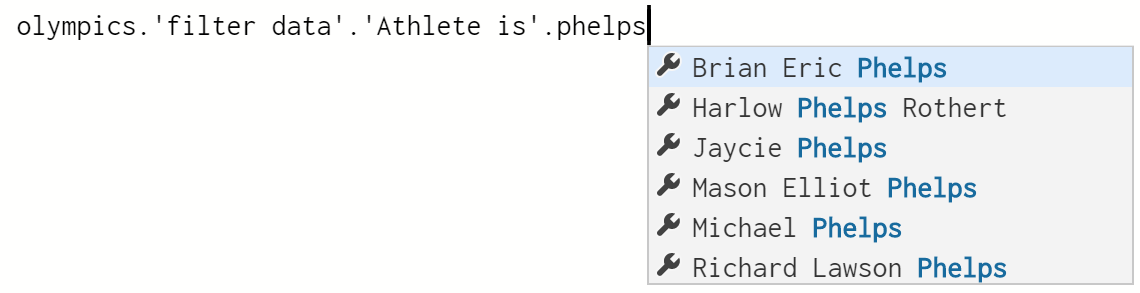
\includegraphics[scale=0.35,trim=0mm 0mm 0mm 0mm,clip]{images/filter.png} % left bottom right top
\end{center}
\caption{Auto-completion offering the available values of the athlete name column}
\label{fig:dot-driven}
\end{figure}

% --------------------------------------------------------------------------------------------------

\subsection{Unifying language constructs with member access}
\label{sec:analysis-dot}

LISP is perhaps the best example of a language that unifies many distinct constructs using a single
form. In LISP, everything is an s-expression, that is, either a list or a symbol. In contrast, 
a typical data processing language uses a number of distinct constructs including indexers (for 
range selection and filtering), method calls (for transformations) and named parameters (for further 
configuration). Consider filtering and sorting:
%
\begin{equation*}
\begin{array}{l}
\ident{data}[\ident{data}[\str{Games}]==\str{Rio (2016)}] \qquad\ball{1}\\
\ident{data}.\ident{filter}(\kvd{fun}~\ident{row}\rightarrow\ident{row}.\ident{Games}=\str{Rio (2016)})\qquad\ball{2}\\
\ident{data}.\ident{sort\_values}(\ident{by}=\str{Gold}, \ident{ascending}=\kvd{False})\qquad\ball{3}\\
\end{array}
\end{equation*}

\noindent
Pandas uses indexers for filtering \ball{1} which can alternatively be written (e.g.~in 
LINQ) using a method taking a predicate as a lambda function \ball{2}. Operations that are 
parameterized only by column name, such as sorting in pandas \ball{3} are often methods with 
named parameters.

We aim to unify the above examples using a single language construct that offers a high-level programming
model and can be supported by modern tooling (as discussed in Section~\ref{sec:analysis-auto}).
Member access provides an extremely simple programming construct that is, in conjunction with
the type provider mechanism, capable of expressing the above data transformations in a uniform way: 
%
\begin{equation*}
\begin{array}{l}
\ident{data}.\qident{sort data}.\qident{by Gold descending}.\ident{then}\qquad\ball{1}\\
\ident{data}.\qident{filter data}.\qident{Games is}.\qident{Rio (2016)}.\ident{then}\qquad\ball{2}\\
\end{array}
\end{equation*}

\noindent
The member names tend to be longer and descriptive. Quoted names appear as \textquotesingle$\ldots$\textquotesingle~in
code, but we typeset them using \qident{...} for readability.
The names are not usually typed by the user (see~Section~\ref{sec:analysis-auto}) and so the
length is not an issue when writing code. The above two examples illustrate two interesting
aspects of our approach. 

\subparagraph{Members, type providers, discoverability.}
When sorting \ball{1} the member that specifies how sorting is done includes the name of the
column. This is possible because the pivot type provider tracks the column names (see 
Section~\ref{sec:columns}) and provides members based on the available columns suitable
for use as sort keys. When filtering \ball{2}, the member \qident{Rio (2016)} is provided based
on the values in the data source (we discuss this further in Section~\ref{sec:pivot-filter}).

These two examples illustrate that member access can be expressive, but it requires huge number
of types with huge number of members. Type providers address this by integration with the type
system (formalized in Section~\ref{sec:foo}) that discovers members lazily. This is why 
approaches based on code generation or pre-processors would not be viable.

Using descriptive member names is only possible when the names are discoverable. The above
code could be executed in a dynamically-typed language that allows custom message-not-understood
handlers, but it would be impossible to get the name right when writing it. Our approach 
relies on discovering names through auto-completion as discussed in Section~\ref{sec:analysis-auto}.

\subparagraph{Expressivity of members.} 
Using member access as the primary mechanism for programming reduces the expressivity of the 
language -- our aim is to create a domain-specific language for data exploration, rather than
a general purpose language\footnote{Designing a general purpose language based on member access
is a separate interesting problem.}. For this purpose, the sequential nature of member accesses 
matches well with the sequential nature of data transformations.

The members provided, for example, for filtering limit the number of conditions that can be 
written, because the user is restricted to choosing one of the provided members.
As illustrated by the case study based on our implementation (Section~\ref{sec:impl}),
this appears sufficient for many common data exploration tasks. The mechanism could be made
more expressive, but we leave this for future work -- for example, the type provider could
accept or reject member names written by the user (as in internet search) rather than providing 
names from which the user can choose (as in web directories).

% --------------------------------------------------------------------------------------------------
 
\begin{figure}
\begin{equation*}
\quad \begin{array}{l}
\qident{drop columns}\\
\quad\rightarrow~\qident{drop Athlete}\\
\quad\rightarrow~\qident{drop Discipline}\\
\quad\rightarrow~\qident{drop Year}\\[0.5em]
\qident{sort data}\\
\quad\rightarrow~\qident{by Athlete}\\
\quad\rightarrow~\qident{by Athlete descending}\\
\quad\rightarrow~\qident{by Discipline}\\
\quad\rightarrow~\qident{by Discipline descending}\\
\end{array}\qquad
\begin{array}{l}
\qident{group data}\\
\quad\rightarrow~\qident{by Athlete}\\
\qquad\quad\rightarrow~\qident{average Year}\\
\qquad\quad\rightarrow~\qident{sum Year}\\[0.5em] 
\quad\rightarrow~\qident{by Year}\\
\qquad\quad\rightarrow~\qident{distinct Athlete}\\
\qquad\quad\rightarrow~\qident{concat Athlete}\\
\qquad\quad\rightarrow~\qident{distinct Discipline}\\
\qquad\quad\rightarrow~\qident{concat Discipline}\\
\end{array}
\end{equation*}
\caption{Subset of members provided by the pivot type provider}
\label{fig:pivot-members}
\end{figure}

% --------------------------------------------------------------------------------------------------
  
\subsection{Tooling and dot-driven development}
\label{sec:analysis-auto}

Source code editors for object-based languages with nominal type systems often provide 
auto-completion for members of objects. This combination works extremely well in practice; the
member list is a complete list of what might follow after typing ``dot'' and it can be easily
obtained for an instance of known type. The fact that developers can often rely on just typing
``dot'' and choosing an appropriate member led to a semi-serious phrase dot-driven development,
that we (equally semi-seriously) adopt in this paper.

Type providers in F\# rely on dot-driven development when navigating through data. When writing code 
to access current temperature $\ident{ldn.Main.Temp}$ in Section~\ref{sec:tps}, the auto-completion
offers various available properties, such as \ident{Wind} and \ident{Clouds} once ``dot'' is typed
after $\ident{ldn.Main}$. Other type providers \cite{inforich} follow a similar pattern. It is worth noting
that despite the use of nominal typing, the names of types rarely explicitly appear in code -- we
do not need to know the name of the type of $\ident{ldn.Main}$, but we need to know its members.
Thus the type name can be arbitrary \cite{fsdata} and is used merely as a lookup key.

The pivot type provider presented in this paper uses dot-driven development for suggesting 
transformations as well as possible values of parameters. This is illustrated in Figure~\ref{fig:dot-driven}
where the user wants to obtain medals of a specific athlete and is offered a list of possible 
names. The editor filters the list as the user starts typing the required name. 

Figure~\ref{fig:pivot-members} lists a subset of the members from the
example in Section~\ref{sec:intro}. After choosing \qident{sort data}, the user is offered 
the possible sorting keys. After choosing \qident{group data}, the user first 
selects the grouping key and then can choose one or more aggregations that can be applied on
other columns of the group. Thus an entire data transformation (such as choosing top 8 athletes
by the number of gold medals) can be constructed using dot-driven development.
  
\subparagraph{Values vs. types.}
As Figure~\ref{fig:dot-driven} illustrates, the pivot type provider sometimes blurs the 
distinction between values and types. In the example in Section~\ref{sec:intro},
\str{Rio (2016)} is a string value in Python, but a statically-typed member \qident{Rio (2016)}
when using the pivot type provider. This is a recurring theme in type provider development\footnote{The
\ident{Individuals} property in the Freebase type provider \cite{inforich} imports values into types in a similar way.}.


Our language supports method calls and so some of the opertaions that are currently exposed as
member access could equally be provided as methods. For example, filtering could be written as 
$\qident{Games is}(\str{Rio (2016)})$. However, the fact that we can offer possible values when
filtering largely simplifies writing of the script for the most 
common case when the user is interested in one of the known values.

Unlike in traditional development, a data scientist doing data exploration often has the entire 
data set available. The pivot type provider uses this when offering possible values for filtering
(Section~\ref{sec:pivot-filter}), but all other operations (Section~\ref{sec:pivot-core}) require 
only meta-data (names and types of columns). Following the example of type providers for structured 
data formats~\cite{fsdata}, the schema could be inferred from a representative sample.

% --------------------------------------------------------------------------------------------------
   
\subsection{Expressing structured logic using members}
\label{sec:analysis-and}

In the motivating example, the \ident{agg} method takes a dictionary that specifies one or more 
aggregates to be calculated over a group. We sum the number of gold medals, but we could also sum
the number of silver and bronze medals, concatenate names of teams for the athlete and perform other 
aggregations. In this case, we provide a nested structure (list of aggregations) as a parameter of 
a single operation (grouping). 

This is an interesting case, because when encoding program as a sequence of member accesses, 
there is no built-in support for nesting. In the pivot type provider, we use the ``then'' design
pattern to provide operations that require nesting. The following example specifies multiple 
aggregations and then sorts data by multiple keys:
%
\begin{equation*}
\begin{array}{l}
\ident{olympics}.\\
\quad\qident{group data}.\qident{by Athlete}.\\
\qquad.\qident{sum Gold}.\qident{sum Silver}.\qident{concat Team}.\ident{then} \qquad\ball{1}\\
\quad.\qident{sort data}.\\
\qquad.\qident{by Gold descending}.\qident{and Silver descending}.\ident{then} \qquad\ball{2}\\
\end{array}
\end{equation*}

\noindent
When grouping, we sum the number of gold and silver medals and concatenates distinct team names~\ball{1}. 
Then we sort the grouped data using two sorting keys \ball{2} -- first by the number of gold 
medals and then silver medals (within a group with the same number of gold medals). 

\subparagraph{The ``then'' pattern.}
Nesting is an essential programming construct and it may be desirable to support it directly in 
the language, but the ``then'' pattern lets us express nesting without language support. In both 
of the cases above, the nested structure is specified by selecting one or more members and then 
ending the nested structure using the \ident{then} member.

In case of grouping, we choose aggregations (\qident{sum Gold}, \qident{concat Team}, etc.) after 
we specify grouping key using \qident{by Athlete}. In case of sorting, we specify the first key
using \qident{by Gold descending} and then add more nested keys using \qident{and Silver descending}.
Thanks to the dot-driven development and the ``then'' pattern, the user is offered possible 
parameter values (aggregations or sorting keys) even when creating a nested structure. We also use
the simple structure of the ``then'' pattern to automatically generate interactive user
interfaces for specifying aggregation and sorting parameters (Section~\ref{sec:impl}).

\subparagraph{Renaming columns.}
The pivot type provider automatically chooses names for the columns obtained as the result of
aggregation. In the above example \ball{1}, the resulting data set will have columns Athlete
(the grouping key) together with Gold, Silver and Team (based on the aggregated columns).
The user cannot currently rename the columns.

In type providers for F\#, renaming of columns could be encoded using methods with static parameters \cite{staticpar} by writing, 
for example, $\ident{g}.\qident{sum Gold as}\langl\str{Total Gold}\rangl()$. In F\#, the value of 
the static parameter (here, \str{Total Gold}) is passed to the type provider, which can use it to
generate the type signature of the method and the return type with member name according to the
value of the static parameter.

% ==================================================================================================

\section{Tracking column names}
\label{sec:columns}

The last difficulty with data scripting discussed in Section~\ref{sec:analysis-why} is that pandas 
(and most other data exploration libraries, even for statically-typed languages) track column names as 
strings at runtime, making code error-prone and auto-complete on column names difficult to support.
Proponents of static typing would correctly point out that column names and their types can be
tracked by a more sophisticated type system. 

In this section, we discuss our approach -- we track column names statically using a mechanism
that is inspired by row types and type state (Section~\ref{sec:columns-row}), however we 
embed the mechanism using type providers into a simple nominal type system (Section~\ref{sec:columns-tp}).
This way, the host language for the pivot type provider can be extremely simple -- and indeed, the
mechanism could be added to languages such as Java or TypeScript with minimal effort. 

% --------------------------------------------------------------------------------------------------

\subsection{Using row types and type state}
\label{sec:columns-row}

There are several common data transformations that modify the structure of the data set and affect
what columns (and of what types) are available. When grouping and aggregating data, the resulting
data set has columns depending on the aggregates calculated. For simplicity, we consider another 
operation -- removing column from the data set. For example, given the Olympic medals data set, we 
can drop \ident{Games} and \ident{Year} columns as follows:
%
\begin{equation*}
  \begin{array}{l}
    \ident{olympics}.\qident{drop columns}.\qident{drop Games}.\qident{drop Year}.\ident{then}
  \end{array}
\end{equation*}

\noindent
Operations that change the type of rows in the data set can be captured using row types~\cite{rowtypes}. 
Row types make it possible to statically track operations on records that add or remove fields
and so they can be used for the typing of operations such as $\qident{drop Year}$.
In addition, we need to annotate type with a form of typestate \cite{typestate} to restrict what operations are available. 
When dropping columns, we first access the \qident{drop columns} member, which sets the state to
a state where we can drop individual columns using \qident{drop $f$}. The \ident{then} member can 
then be used to complete the operation and choose another transformation.

To illustrate tracking of columns using row types and type state, consider a simple language with
variables (representing external data sources) and member access. Types can be either primitive 
types $\alpha$, types annotated with a type state \ident{lbl} or row type with fields $f$:

\noindent
\begin{equation*}
\begin{array}{rcl}  
e&=&v \lsep e.N\\
\tau&=&\alpha \lsep \tau_\ident{lbl} \lsep [f_1\!:\!\tau_1, \ldots, f_n\!:\!\tau_n] 
\end{array}  
\end{equation*}

\noindent
Typing rules for members that are used to drop columns are shown in Figure~\ref{fig:fancy-types}.
When \qident{drop columns} is invoked on a record, the type is annotated with a state \ident{drop}
(\emph{drop-start}) indicating that individual columns may be dropped. The \ident{then} 
operation (\emph{drop-then}) removes the state label. Individual members can be removed using
\qident{drop $f_i$} and the (\emph{drop-col}) rule ensures the dropped column is available in the
input row type and removes it.

Other data transformations could be type checked in a similar way, but there are two drawbacks.
First, row types and typestate (although relatively straightforward) make the host language more
complex. Second, rules such as (\emph{drop-col}) make auto-completion more difficult, because the
editor needs to understand the rules and calculate what members may be invoked. This is a distinct
operation from type checking and type inference (which operate on complete programs) that needs 
to be formalized and implemented.

% --------------------------------------------------------------------------------------------------

\begin{figure}

\begin{equation*}
\inference[(\emph{drop-start})~]
  {\Gamma \vdash e : [f_1\!:\!\tau_1, \ldots, f_n\!:\!\tau_n]}
  {\Gamma \vdash e.\qident{drop columns}: [f_1\!:\!\tau_1, \ldots, f_n\!:\!\tau_n]_{\ident{drop}}}
\end{equation*}

\begin{equation*}
\inference[(\emph{drop-col})~]
  {\Gamma \vdash e : [f_1\!:\!\tau_1, \ldots, f_n\!:\!\tau_n]_{\ident{drop}}}
  {\Gamma \vdash e.\qident{drop~$f_i$}: [f_1\!:\!\tau_1, \ldots, f_{i-1}\!:\!\tau_{i-1}, f_{i+1}\!:\!\tau_{i+1}, \ldots, f_n\!:\!\tau_n ]_{\ident{drop}}}
\end{equation*}

\begin{equation*}
\inference[(\emph{drop-then})~]
  {\Gamma \vdash e : [f_1\!:\!\tau_1, \ldots, f_n\!:\!\tau_n]_{\ident{drop}}}
  {\Gamma \vdash e.\qident{then}: [f_1\!:\!\tau_1, \ldots, f_n\!:\!\tau_n]}
\end{equation*}


\caption{Tracking available column names with row types and type state}
\label{fig:fancy-types}
\end{figure}

% --------------------------------------------------------------------------------------------------

\subsection{Using the pivot type provider}
\label{sec:columns-tp}

In our approach, the information about available fields is used by the pivot type provider to provide
types with appropriate members. This is hidden from the host language, which only sees class types.
Provided class definitions consist of a constructor and members: 
%
\begin{equation*}
\begin{array}{rcl}
 l &=& \kvd{type}~C(x:\tau) = \overline{m} \\
 m &=& \kvd{member}~N:\tau= e
\end{array}
\end{equation*}

\noindent
During type checking, the type system keeps track of a lookup of provided class definitions $L$. 
Checking member access is then just a matter of finding the corresponding class definition and
finding the member type:
%
\begin{equation*}
\inference[(\emph{member})~]
  {L; \Gamma \vdash e : C & L(C)=\kvd{type}~C(x:\tau) = ..\;\kvd{member}~N_i : \tau_i = e_i\;..}
  {L; \Gamma \vdash e.N_i:\tau_i}
\end{equation*}

\noindent
The rule, adapted from \cite{fsdata}, does not capture laziness of type providers that is 
important for the pivot type provider (where the number of provided classes is potentially 
infinite). We discuss this aspect in Section~\ref{sec:foo}.

Using type providers and nominal type system hides knowledge about fields available
in the data set. However, for types constructed by the pivot type provider, we can define a 
mapping \ident{fields} that returns the fields available in the data set represented by the 
class. The type provider encodes the logic expressed in Section~\ref{sec:columns-row} in the
following sense:

\begin{rmrk}[Encoding of fancy types]
\label{thm:encoding-fancy}
If $\Gamma\vdash e:[f_1\!:\!\tau_1, \ldots, f_n\!:\!\tau_n]$ using a type system defined in 
Figure~\ref{fig:fancy-types} and $\Gamma\vdash e:C$ using nominal typing and $C$ is a type 
provided by the pivot type provider then $\ident{fields}(C) = \{ f_1\mapsto\tau_1, \ldots, f_n\mapsto\tau_n \}$.
\end{rmrk}

\noindent
In the following two sections, we focus on formalizing the pivot type provider and the nominally 
typed host language. We define the \ident{fields} predicate in Section~\ref{sec:pivot-prop} and use it 
to prove properties of the pivot type provider.

We do not fully develop the type system based on fancy types sketched in Section~\ref{sec:columns-row}.
However, the remark illustrates one interesting aspect of our work -- the type provider 
mechanism makes it possible to express safety guarantees that would normally require row types and 
typestate in a simple nominally typed language. In a similar way, type providers have been used
to encode session types \cite{sessiontp}, suggesting that this is a generally useful approach.

% ==================================================================================================

\begin{figure}

\begin{equation*}
\begin{array}{rclll}
  D & = & \multicolumn{3}{l}{ 
    \{f_1\mapsto \vect{v_{1,1},\ldots,v_{1,r}}, \ldots, f_n\mapsto \vect{v_{n,1},\ldots,v_{n,r}}\} 
  }\\[0.5em]
  e & = & \Pi_{f_1, \ldots, f_n} (e) &&\textnormal{Projection -- select specified column names}\\
   & \lsep & \sigma_\varphi (e) &&\textnormal{Selection -- filter rows by given predicate}\\
   & \lsep & \tau_{f_1\mapsto\omega_1, \ldots, f_n\mapsto\omega_n}(e) &&\textnormal{Sorting -- sort by specified columns}\\
   & \lsep & \Phi_{f, \rho_1/f_1, \ldots, \rho_n/f_n} (e) &&\textnormal{Grouping -- group by and calculate aggregates}
   \\[0.5em]
  \omega & = & \ident{desc}\lsep\ident{asc}  &&\textnormal{Sort order -- descending or ascending}\\
  \rho & = & \ident{count}  &&\textnormal{Count number of rows in the group}\\
   & \lsep & \ident{sum}~f  &&\textnormal{Sum numerical values of the column $f$}\\
   & \lsep & \ident{dist}~f &&\textnormal{Count number of distinct values of the column $f$}\\
   & \lsep & \ident{conc}~f &&\textnormal{Concatenate string values of the column $f$}\\
\\
\end{array} 
\end{equation*}

\vspace{-1.5em}
\caption{Relational algebra with values, sorting and aggregation}
\label{fig:foo-rel}
\end{figure}

% --------------------------------------------------------------------------------------------------

\begin{figure}
\vspace{-1em}
\begin{equation*}
\begin{array}{l}
\Pi_{f_{p(1)}, \ldots, f_{p(m)}} \{f_1\mapsto \vect{v_{1,1},\ldots,v_{1,r}}, \ldots, f_n\mapsto \vect{v_{n,1},\ldots,v_{n,r}}\} \leadsto \\
  \quad \{f_{p(1)}\mapsto \vect{v_{p(1),1},\ldots,v_{p(1),r}}, \ldots, f_{p(m)}\mapsto \vect{v_{p(m),1},\ldots,v_{p(m),r}}\}  
\\
\\
\sigma_\varphi \{f_1\mapsto \vect{v_{1,1},\ldots,v_{1,r}}, \ldots, f_n\mapsto \vect{v_{n,1},\ldots,v_{n,r}}\} \leadsto\\
  \quad \{f_1\mapsto \vect{\ldots, v_{1,j}, \ldots}, \ldots, f_n\mapsto \vect{\ldots, v_{n,j},\ldots}\}
  \qquad (\forall j.\;\varphi\, \{f_1\mapsto v_{1,j}, \ldots, f_n\mapsto v_{n,j}\})
\\
\\
\tau_{f_{p(1)}\mapsto\omega_1, \ldots, f_{p(m)}\mapsto\omega_m} \{f_1\mapsto \vect{v_{1,1},\ldots,v_{1,r}}, \ldots, f_n\mapsto \vect{v_{n,1},\ldots,v_{n,r}}\} \leadsto\\
  \quad \{f_1\mapsto \vect{v_{1,q(1)},\ldots,v_{1,q(r)}}, \ldots, f_n\mapsto \vect{v_{n,q(1)},\ldots,v_{n,q(r)}}\} 
  \quad \textnormal{where $q$ permutation}\\
  \qquad \textnormal{such that}~\forall i, j.~i\leq j\implies(u_{1,i}, \ldots, v_{m,i}) \leq (v_{1,j}, \ldots, v_{m,j})~ \textnormal{where}\\
  \qquad \quad u_{k,l}=v_{p(k),q(l)} \quad \,~~(\textnormal{when}~\omega_k=\ident{asc}) \\
  \qquad \quad u_{k,l}=-v_{p(k),q(l)} \quad (\textnormal{when}~\omega_k=\ident{desc})
  \\
  \\
\Phi_{f_i, \rho_1/f_1', \ldots, \rho_m/f_m'} \{f_1\mapsto \vect{v_{1,1},\ldots,v_{1,r}}, \ldots, f_n\mapsto \vect{v_{n,1},\ldots,v_{n,r}}\} \leadsto\\
  \quad \{f_1' \mapsto a_1, \ldots, f_m'\mapsto a_m, f_i\mapsto b \} 
  \quad \textnormal{where}\\
  \qquad \{g_1,\ldots,g_s\}=\{\{l~|~k\in 1\ldots r, ~v_{i,l}=v_{i,k}\}, ~l\in 1\ldots r\} \\
  ~~\begin{array}{ll}    
    \qquad b = \vect{v_{i,k_1},\ldots,v_{i, k_s}} & \textnormal{where}~k_j \in g_j \\
    \qquad a_i = \vect{|g_1|, \ldots, |g_s|}  & \textnormal{when}~\rho_i = \ident{count} \\
    \qquad a_i = \vect{\Sigma_{k\in g_1}v_{j,k}, \ldots, \Sigma_{k\in g_s}v_{j,k}} & \textnormal{when}~\rho_i = \ident{sum}~f_j \\
    \qquad a_i = \vect{\Pi_{k\in g_1}v_{j,k}, \ldots, \Pi_{k\in g_s}v_{j,k}}   & \textnormal{when}~\rho_i = \ident{conc}~f_j \\
    \qquad a_i = \vect{|\{v_{j,k}\,|\, k\in g_1\}|, \ldots, |\{v_{j,k}\,|\, k\in g_s\}|}  & \textnormal{when}~\rho_i = \ident{dist}~f_j \\
  \end{array}\\
\end{array}
\end{equation*}

\caption{Vector-based semantics for operations of the extended relational algebra}
\label{fig:foo-relsem}
\end{figure}

% --------------------------------------------------------------------------------------------------

\section{Formalising the host language and runtime}
\label{sec:foo}

Type providers often provide a thin type-safe layer over richer untyped runtime components. In case 
of providers for data access (Section~\ref{sec:tps}), the untyped runtime component performs lookups
into external data sources. In case of the pivot type provider, the untyped runtime component 
is a relational algebra modelling data transformations. We formalize the relational algebra in 
Section~\ref{sec:foo-rel}, followed by the object-based host language in Section~\ref{sec:foo-foo}.

\subsection{Relational algebra with vector semantics}
\label{sec:foo-rel}

The focus of our work is on data aggregation and so we use a form of relational algebra with 
extensions for grouping and sorting \cite{relalg,dbsys}. The syntax is defined in Figure~\ref{fig:foo-rel}.
We write $f$ for column (field) names and we include definition of a data value $D$, which maps
column names to vectors of length $r$ storing the data (values $v$ are defined below).
Aside from standard projection $\Pi$ and selection $\sigma$, our algebra includes sorting 
$\tau$ which takes one or more columns forming the sort key (with sort order $\omega$)
and aggregation $\Phi$, which requires a single grouping key and several aggregations together with 
names of the new columns to be returned.

The semantics of the algebra is given in Figure~\ref{fig:foo-relsem}. We use vector-based semantics
to support sorting and duplicate entries, but otherwise the formalization captures the usual
behaviour. In projection and sorting, we write $f_{p(1)}, \ldots, f_{p(m)}$ to refer to a selection
of fields from $f_1, \ldots, f_n$. Assuming $m\leq n$, $p$ can be seen as a mapping from $\{1\ldots m\}$
to a subset of $\{1\ldots n\}$. In selection, $\varphi$ is a predicate applied to a mapping from 
column names to values. In sorting, we assume that there is a permutation on row indices $q$ such
that the tuples obtained by selecting values according to the given sort key are ordered. The 
auxiliary definition $u_{k,l}$ negates the number to reverse the sort order when descending order
is required.

The most complex operation is grouping. We need to group data by the value of the column $f_i$ and
then apply aggregations $\rho_1,\ldots,\rho_m$. To do this, we first obtain a set of groups $g_1,\ldots, g_s$
where each group represents a set of indices of rows belonging to each group. For a given group 
$g_i$ we can then obtain values of column $j$ for rows in the group as $\{v_{j,k}\,|\, k\in g_i\}$.
This is used to calculate the resulting data set -- the field $f_i$ becomes a new column formed
by the group keys (obtained by picking one of the indices from $g_j$ for each group); other fields
are calculated by aggregating data in various ways -- $|g_i|$ gives the number of rows in the group,
$\Sigma$ sums numerical values and $\Pi$ (a slight notation abuse) concatenates string values. 

% --------------------------------------------------------------------------------------------------

\begin{figure}
\vspace{-1em}
\begin{equation*}
\begin{array}{rcl}
  v &=& C(v)\,\, \lsep \ident{series}\langl \tau_1, \tau_2 \rangl(v)\; \lsep n \lsep s \lsep D \\
  e &=& C(e)\,\, \lsep \ident{series}\langl \tau_1, \tau_2 \rangl(e)\;\, \lsep x \lsep v \lsep e.N \lsep \ldots\\
  E &=& C(E) \lsep \ident{series}\langl \tau_1, \tau_2 \rangl(E)\, \lsep E.N \\
    &|& \Pi_{f_1, \ldots, f_n}(E) \lsep \sigma_\varphi(E) \lsep \tau_{f_1, \ldots, f_n}(E) \lsep \Phi_{f, \rho_1/f_1, \ldots, \rho_m/f_m} (E) \\
    \\
 \tau &=& C \lsep \kvd{num} \lsep \kvd{string} \lsep \ident{series}\langl \tau_1, \tau_2 \rangl \lsep \ident{Query}\\
 l &=& \kvd{type}~C(x:\tau) = \overline{m} \\
 m &=& \kvd{member}~N:\tau= e
\end{array}
\end{equation*}
\vspace{-1.85em}

\[
\inference[(\emph{member})~]
{ L(C) = (\kvd{type}~C(x:\tau)= \ldots~\kvd{member}~N_i : \tau_i = e_i~\ldots), L'}
{ (C(v)).N_i \leadsto_L e_i[x \leftarrow v] }\\
\]
\vspace{-3.15em}

\[
\inference[(\emph{context})~]
{e \leadsto_L e'}
{E[e] \leadsto_L E[e']}
\]
\caption{Syntax and remaining reduction rules of the Foo calculus}
\label{fig:foo-syntax}
\end{figure}

% --------------------------------------------------------------------------------------------------

\subsection{Foo calculus with lazy context}
\label{sec:foo-foo}

We model the host language using a variant of the Foo calculus \cite{fsdata}. The core of the calculus models
a simple object-based language with objects and members. The syntax of the language is shown in
Figure~\ref{fig:foo-syntax}. The relational algebra defined in Figure~\ref{fig:foo-rel} is included
in the Foo calculus as a model of the runtime components of the pivot type provider -- the values
include the data value $D$ and the expressions include all the operations of the relational algebra.

The Foo calculus includes two special types. \ident{Query} is a type of data and queries 
constructed using the relational algebra. The type $\ident{series}\langl \tau_1, \tau_2 \rangl$ 
models a type-safe data series mapping keys of type $\tau_1$ to values of type $\tau_2$ that
can be used, for example, as input for a charting library. A series is a typed wrapper over a 
\ident{Query} value and the proofs in Section~\ref{sec:pivot-prop} show that a series obtained 
from the pivot type provider contains keys and values of matching~types.

\subparagraph{Reduction rules.} The reduction relation $\leadsto_L$ is parameterized by a function
$L$ that maps class names to class definitions, together with nested classes associated with the
class definition (used during type checking as discussed below). The map is not used in the 
reduction rules for the relational algebra, given in Figure~\ref{fig:foo-relsem} and so it was 
omitted there.

The remaining reduction rules are given in Figure~\ref{fig:foo-syntax}. The (\emph{member}) rule 
performs lookup using $L(C)$ to find the definition of the member that is being accessed and then
it reduces member access by substituting the evaluated constructor argument $v$ for a variable $x$.
We assume standard capture-avoiding substitution $[x\leftarrow v]$. The rule ignores the nested 
class definitions $L'$. The (\emph{context}) rule performs reduction in an evaluation context $E$.

\subparagraph{Type checking.} One interesting aspect of type checking with type providers is that
type providers can provide potentially infinite number of types. The types are provided 
lazily as the type checker explores parts of the type space used by the program \cite{inforich}. 
Consider:
%
\begin{equation*}
\ident{olympics}.\qident{group data}.\qident{by Athlete}.\qident{sum Gold}.\ident{then}
\end{equation*}

\noindent
The type checker initially knows the type of $\ident{olympics}$ is a class $C_1$ with member 
$\qident{group data}$ and it knows that the type of this member is $C_2$. However, it only needs to 
obtain full definition of $C_2$ when checking the member $\qident{by Athlete}$. Types of other 
members of $C_1$ remain unevaluated. This aspect of type
providers have been omitted in previous work \cite{fsdata,liteq}, but it is necessary for the pivot type provider.
The typing rules given are written as:
%
\begin{equation*}
L_1; \Gamma \vdash e : \tau; L_2
\end{equation*}

\noindent
The judgement states that given class definitions $L_1$ and a variable context $\Gamma$, the type
of expression $e$ is $\tau$ and the type checking evaluated class definitions that are
now included in~$L_2$. The resulting context obtained by type checking contains all definitions
that may be needed when running the program and is passed to the reduction operation $\leadsto_{L}$.

The structure of class definitions $L$ is a function mapping a class name 
$C$ to a pair consisting of the definition and a function that provides definitions of 
delayed classes: 
%
\begin{equation*}
L(C) = \kvd{type}~C(x:\tau) = \overline{m}, L'
\end{equation*}

\noindent
The class $C$ may use classes defined in $L$, but also delayed classes from $L'$. This models 
laziness as $L'$ is a function that may never be evaluated. Since $L$ is potentially infinite, we 
cannot check class definitions upfront as in typical object calculi \cite{objects}. Instead, we check that 
that members are well typed as they appear in the source code, which matches the behaviour of F\# 
type providers. In general, this means that $L$ may contain classes with incorrectly typed 
members. We prove that this is not the case for the pivot type provider (Section~\ref{sec:pivot-prop}).

The rules that define type checking are shown in Figure~\ref{fig:foo-typecheck}. The two rules
that force the discovery of new classes are (\emph{new}) and (\emph{member}). In (\emph{new}), we
find the class definition and delayed classes using $L_2(C)$. We treat functions as sets and 
join $L_2$ with delayed classes defined by $L$ using $L_2 \cup L$. In (\emph{member}), we obtain
the class definition and discover delayed classes in the same way, but we also check that the body
of the member is well-typed.

% --------------------------------------------------------------------------------------------------

\begin{figure}[t]
\vspace{-0.5em}
\[
\inference[(\emph{num})~]{}{L; \Gamma \vdash n : \kvd{num}; L }
\quad
\inference[(\emph{string})~]{}{L; \Gamma \vdash s : \kvd{string}; L}
\quad
\inference[(\emph{var})~]{}{L; \Gamma, x:\tau\vdash x:\tau; L}
\]
\vspace{-1.75em}

\[
\inference[(\emph{data})~]
  {L; \Gamma \vdash v_{i,j} : \tau;L \quad \tau \in \{ \kvd{num}, \kvd{string} \}}
  {L; \Gamma \vdash \{f_1\mapsto \vect{v_{1,1},\ldots,v_{1,r}}, \ldots, f_n\mapsto \vect{v_{n,1},\ldots,v_{n,r}}\} : \ident{Query};L }
\]
\vspace{-1.75em}

\[
\inference[(\emph{proj})~]
  {L_1; \Gamma\vdash e : \ident{Query}; L_2}
  {L_1; \Gamma\vdash \Pi_{f_1, \ldots, f_n} (e) : \ident{Query}; L_2}
\qquad\inference[(\emph{sort})~]
  {L_1; \Gamma\vdash e : \ident{Query}; L_2}
  {L_1; \Gamma\vdash \tau_{f_1, \ldots, f_n}(e): \ident{Query}; L_2}
\]

\[
\inference[(\emph{sel})~]
  {L_1; \Gamma\vdash e : \ident{Query}; L_2}
  {L_1; \Gamma\vdash \sigma_\varphi (e) : \ident{Query}; L_2}
\qquad
\inference[(\emph{group})~]
  {L_1; \Gamma\vdash e : \ident{Query}; L_2}
  {L_1; \Gamma\vdash \Phi_{f, \rho_1/f_1, \ldots, \rho_n/f_n}(e): \ident{Query}; L_2}
\]
\vspace{-1.75em}

\[
\inference[(\emph{series})~]
  {L_1; \Gamma\vdash e : \ident{Query}; L_2}
  {L_1; \Gamma\vdash \ident{series}\langl \tau_1, \tau_2 \rangl(e) : \ident{series}\langl \tau_1, \tau_2 \rangl; L_2}
\]
\vspace{-1.75em}

\[
\inference[(\emph{new})~]
  {L_1; \Gamma \vdash e : \tau, L_2 & L_2(C) = (\kvd{type}~C(x:\tau) = \ldots),L}
  {L_1; \Gamma \vdash C(e) : C; L_2 \cup L}
\]
\vspace{-1.75em}

\[
\inference[(\emph{member})~]
  {L_1; \Gamma \vdash e : C; L_2 \qquad L_2\cup L; \Gamma,x:\tau \vdash e_i : \tau_i; L_3 \\
   L_2(C)=(\kvd{type}~C(x:\tau) = ..\;\kvd{member}~N_i : \tau_i = e_i\;..), L }
  {L_1; \Gamma \vdash e.N_i:\tau_i; L_3}
\]
\vspace{-0.5em}
\caption{Type-checking of Foo expressions with lazy context}
\label{fig:foo-typecheck}
\end{figure}

% --------------------------------------------------------------------------------------------------

The rules for primitive types and variables are standard. Input data (\emph{data}) is of type 
\ident{Query} and all the operations of relational algebra take \ident{Query} input and 
produce \ident{Query} results. An untyped \ident{Query} value can be converted into a 
series (\emph{series}) of any type, akin to the boundary between static and dynamic typing 
in gradually typed languages~\cite{gradual}. When provided by the pivot type provider, 
the operation produces series with values of correct~types.

% --------------------------------------------------------------------------------------------------

\begin{figure}
\begin{equation*}
\begin{array}{ll}
\ident{pivot}(F) = C, \{ C \mapsto (l, L_1 \cup \ldots \cup L_4) \}\qquad\ball{1}\\[0.5em]
\quad l = \kvd{type}~C(x:\ident{Query}) = \\
\qquad \qquad \kvd{member}~\qident{drop columns} : C_1 = C_1(x) &\textnormal{where}~C_1, L_1 = \ident{drop}(F)\\
\qquad \qquad \kvd{member}~\qident{sort data} : C_2 = C_2(x) &\textnormal{where}~C_2, L_2 = \ident{sort}(F)\\
\qquad \qquad \kvd{member}~\qident{group data} : C_3 = C_3(x) &\textnormal{where}~C_3, L_3 = \ident{group}(F)\\
\qquad \qquad \kvd{member}~\qident{get series} : C_4 = C_4(x) &\textnormal{where}~C_4, L_4 = \ident{get-key}(F)\\
\\
\ident{get-key}(F) = C, \{ C \mapsto (l, \bigcup L_f)\}\qquad\ball{2} \\[0.25em]
\quad l = \kvd{type}~C(x:\ident{Query}) = &\forall f\in\dom(F)~\textnormal{where} \\
\qquad \qquad \kvd{member}~\qident{with key $f$} : C_f = C_f(x) &\quad C_f, L_f = \ident{get-val}(F, f)\\
\\
\ident{get-val}(F, f_k) = C, \{ C \mapsto (l, \{\}) \}\qquad\ball{3} \\[0.25em]
\quad l = \kvd{type}~C(x:\ident{Query}) = &\forall f\in\dom(F)\setminus\{f_k\}~\textnormal{where} \\
\qquad \qquad \kvd{member}~\qident{and value $f$} : \ident{series}\langl\tau_k, \tau_v\rangl = &\quad  \tau_k = F(f_k),~ \tau_v = F(f) \\
\qquad \qquad \quad \ident{series}\langl\tau_k, \tau_v\rangl(\Pi_{f_k, f}(x))\qquad\ball{4}
\end{array}
\end{equation*}

\caption{Pivot type provider -- entry-point type and accessing transformed data}
\label{fig:tp-main}
\end{figure}

% ==================================================================================================

\section{Formalising the pivot type provider}
\label{sec:pivot}

A type provider is an executable component called by the compiler and the editor to 
provide information about types on demand. In our formalization, we follow the 
style of Petricek et al. \cite{fsdata}, but we add laziness as discussed in Section~\ref{sec:foo-foo}.
We model the core operations (dropping columns, grouping and sorting) in Section~\ref{sec:pivot-core}
and refine the model to include filtering Section~\ref{sec:pivot-filter}.
For simplicity we omit paging, which does not affect the shape of data.

% --------------------------------------------------------------------------------------------------

\subsection{Pivot type provider}
\label{sec:pivot-core}

A type provider is a function that takes static parameters, such as schema of the input data set, 
and returns a class name $C$ together with a mapping that defines the body of the class and 
definitions of delayed classes $L$ that may be used by the members of the class $C$. 
In our case, the schema $F$ is a mapping from field names to field types:
%
\begin{equation*}
\begin{array}{l}
\ident{pivot}(F) = C, \{ C \mapsto (\kvd{type}~C(x:\ident{Query}) = \ldots,L) \} \quad \textnormal{where}~F=\{ f_1 \mapsto \tau_1, \ldots, f_n \mapsto \tau_n \}
\end{array}
\end{equation*}
%
The class $C$ provided by the pivot type provider has a constructor taking \ident{Query}, which 
represents the, possibly already partly transformed, input data set. It generates members that
allow the user to refine the query and access the data. The type provider is defined using several
helper functions discussed in the rest of this section.

\subparagraph{Entry-point and data access.} Figure~\ref{fig:tp-main} shows three of the functions
defining the pivot type provider. The \ident{pivot} function \ball{1} defines the entry-point type, 
which lets the user choose which operation to perform before specifying parameters of the operation. 
This is the type of \ident{olympics} in the examples throughout this paper. The definition generates 
a new class $C$ with members that wrap the input data in delayed classes generated by other parts
of the type provider. The result of \ident{pivot} is the class name $C$ together with definition of 
the class and delayed generated types. The definition is a function that only needs to be evaluated 
when a program accesses a member of the class $C$, modelling the laziness of the type provider.
In the implementation, we return the name $C$ together with a function that computes the definition 
of the class when the type checker needs to inspect the body.

The \ident{get-key} \ball{2} and \ident{get-val} \ball{3} functions provide members that can be used 
to choose two columns from the data set as keys and values and obtain the resulting data set as a 
value of type $\ident{series}\langl \tau_1, \tau_2 \rangl$. For example, the following expression 
has a type $\ident{series}\langl \kvd{string}, \kvd{num} \rangl$:
%
\begin{equation*}
\begin{array}{l}
\ident{olympics}.\qident{get series}.\qident{with key Athlete}.\qident{and value Year}
\end{array}
\end{equation*}

\noindent
The \ident{get-key} function generates a class with one member for each field in the data set.
The returned class $C_f$ is generated by \ident{get-val} and lets the user choose any of the 
remaining fields as the value. The key and value columns are then selected using $\Pi_{f_k,f}$ \ball{4}.
The series is then created with a data set containing only the key and value columns (we assume 
the order of columns is preserved). Creating a series does not statically enforce that the 
data set has the right structure, but the properties discussed in Section~\ref{sec:pivot-prop} show 
that series obtained from the pivot type provider is constructed correctly.

% --------------------------------------------------------------------------------------------------

\begin{figure}
\begin{equation*}
\begin{array}{ll}
\ident{drop}(F) = C, \{ C \mapsto (l, L' \cup \bigcup L_f) \}\qquad\ball{1}\\[0.5em]
~ l = \kvd{type}~C(x:\ident{Query}) = &\forall f \in \dom(F)~\textnormal{where}~C_f, L_f = \ident{drop}(F')\\
\quad \qquad \kvd{member}~\qident{drop $f$} : C_f = C_f(\Pi_{\ident{dom}(F')}(x)) & \quad\textnormal{and}~ F' = \{ f'\mapsto\tau'\in F, f' \neq f\}\\
\quad \qquad \kvd{member}~\ident{then} : C' = C'(x)\qquad\ball{2}                 &\textnormal{where}~C', L' = \ident{pivot}(F)\\
\\[0.5em]
\ident{sort}(F) = C, \{ C \mapsto (l, \bigcup L_f \cup \bigcup L'_f) \}\qquad\ball{3}\\[0.25em]
~ l = \kvd{type}~C(x:\ident{Query}) = &\forall f\in\{f~|~F(f)=\kvd{num} \},~\textnormal{where} \\
\quad \qquad \kvd{member}~\qident{by $f$ desc} : C_f = C_f(x) &\quad C_f, L_f = \ident{sort-and}(F, \vect{f \mapsto \ident{desc}})\\
\quad \qquad \kvd{member}~\qident{by $f$ asc} : C'_f = C'_f(x) &\quad C'_f, L'_f = \ident{sort-and}(F, \vect{f \mapsto \ident{asc}})\\
\\[1em]
\multicolumn{2}{l}{ \ident{sort-and}(F,\vect{s_1,\ldots,s_n}) = C, \{ C \mapsto (l, \bigcup L_f \cup \bigcup L'_f \cup L') \}\qquad\ball{4} }\\[0.25em]
~ l = \kvd{type}~C(x:\ident{Query}) = &\hspace{-4em}\forall f\in\{f~|~F(f)=\kvd{num}, \,\nexists i.s_i=f'\mapsto\omega\wedge f'=f\}\\
\quad \qquad \kvd{member}~\qident{$f$ desc} : C_f = C_f(x) &\hspace{-2em} C_f, L_f = \ident{sort-and}(F, \vect{s_1,..,s_n, f \mapsto \ident{desc}})\\
\quad \qquad \kvd{member}~\qident{$f$ asc} : C'_f = C'_f(x) &\hspace{-2em} C'_f, L'_f = \ident{sort-and}(F, \vect{s_1,..,s_n, f \mapsto \ident{asc}})\\
\quad \qquad \kvd{member}~\ident{then} : C' = C'(\tau_{s_1,\ldots,s_n}(x))  &\hspace{-2em}\textnormal{where}~C', L' = \ident{pivot}(F)\qquad ~~\ball{5}\\
\end{array}
\end{equation*}

\caption{Pivot type provider -- dropping columns and sorting data}
\label{fig:tp-ds}
\end{figure}

% --------------------------------------------------------------------------------------------------

\subparagraph{Dropping columns and sorting.} Functions that provide types for the 
\qident{drop columns} and \qident{sort data} members are defined in Figure~\ref{fig:tp-ds}.
The \ident{drop} function \ball{1} builds a new type that lets the user drop any of the available columns.
The resulting type $C_f$ is recursively generated by \ident{drop} so that multiple columns can 
be dropped before completing the transformation using the \ident{then} operation \ball{2}, whose 
return type is generated using the main \ident{pivot} function. Note that columns removed from the 
schema $F'$ match the columns removed from the data set at runtime  
using $\Pi_{\dom(F')}$.

Types for defining the sorting transformation are split between two functions; \ident{sort}~\ball{3} 
generates type for choosing the first sorting key and \ident{sort-and}~\ball{4} lets the user add more
keys. For space reasons, we abbreviate \ident{ascending} and \ident{descending} as \ident{asc} and
\ident{desc} in the generated member names and we omit \ident{and} in name of further keys such as 
\qident{and Gold descending}.

The members are restricted to numerical columns (by checking $F(f)=\kvd{num}$).
The sort keys are kept as a vector. The \ident{sort} operation creates a singleton vector;
\ident{sort-and} appends a new key to the end and the \ident{then} member \ball{5} generates code 
that passes the collected sort keys to the $\tau$ operation of the relational algebra.
When generating members for adding further sort keys, we exclude the columns that are used
already (by checking that the column $f$ does not match column name of any of the existing 
keys $\nexists i.\,s_i = f'\mapsto\omega$). 

% --------------------------------------------------------------------------------------------------

\begin{figure}
\begin{equation*}
\hspace{-1.5em}
\begin{array}{ll}
\ident{group}(F) = C, \{ C\mapsto (l, \bigcup L_f) \}\quad\ball{1} \\[0.25em]
~ l = \kvd{type}~C(x:\ident{Query}) = &\hspace{-2.5em}\forall f\in\dom(F)~\textnormal{where} \\
\quad \qquad \kvd{member}~\qident{by $f$} : C_f = C_f(x) &\hspace{-2.5em}\quad C_f, L_f = \ident{agg}(F, f, \{ f \mapsto F(f) \}, \emptyset)~~\ball{2}\\
\\[0.5em]
\multicolumn{2}{l}{ \ident{agg}(F,f,G,S) = C, \{C\mapsto (l, \bigcup L_f \cup \bigcup L'_f \cup\bigcup L''_f\cup L'\cup L'') \}\quad\ball{3}}\\[0.25em]
~ l = \kvd{type}~C(x:\ident{Query}) = &\forall f\in\dom(F)\setminus\dom(S)\\
\quad \qquad \kvd{member}~\qident{sum $f$} : C'_f = C'_f(x) & \quad \textnormal{when}~F(f)=\kvd{num}\quad\ball{4} \\
\quad \qquad \kvd{member}~\qident{concat $f$} : C''_f = C''_f(x) & \quad \textnormal{when}~F(f)=\kvd{string}\quad\ball{5} \\
\quad \qquad \kvd{member}~\qident{count all} : C' = C'(x) & \quad \textnormal{when}~\ident{Count}\notin G\quad\ball{6} \\
\quad \qquad \kvd{member}~\qident{distinct $f$} : C_f = C_f(x)  \\
\quad \qquad \kvd{member}~\ident{then} : C'' = C''(\Phi_{f, \rho_1/f_1, \ldots, \rho_n/f_n}(x)) &\textnormal{where}~\{\rho_1/f_1,\ldots,\rho_n/f_n\}=S\quad\ball{7} \\[0.5em]
\qquad  \textnormal{where}\\[0.5em]
\multicolumn{2}{l}{
~\,\qquad \begin{array}{l}
 C_f, L_f = \ident{agg}(F,f, G\cup\{ f \mapsto \kvd{num}\}, S\cup\{\ident{dist}~f/f\} )\\
 C'_f, L'_f = \ident{agg}(F,f, G\cup\{ f \mapsto \kvd{num} \}, S\cup\{\ident{sum}~f/f\})\\
 C''_f, L''_f = \ident{agg}(F,f, G\cup\{ f \mapsto \kvd{string} \}, S\cup\{\ident{conc}~f/f\})\\
 C', L' = \ident{agg}(F,f, G\cup\{ \ident{Count}\mapsto\kvd{int} \}, S\cup{\ident{count}/\ident{Count}})\\
 C'', L'' = \ident{pivot}(G)
\end{array} 
}
\end{array}
\end{equation*}

\caption{Pivot type provider -- grouping and aggregation}
\label{fig:tp-group}
\end{figure}

% --------------------------------------------------------------------------------------------------

\subparagraph{Grouping and aggregation.} The final part of the pivot type provider is defined in
Figure~\ref{fig:tp-group}. The \ident{group} function \ball{1} generates a class that lets the user 
select a column to use as the grouping key and \ident{agg} is used to provide aggregates that can be 
calculated over grouped data. The \ident{agg} function \ball{3} takes the schema of the input data 
set $F$, column $f$ to be used as the group key, a schema of the data set that will be produced as 
the result $G$ and a set of aggregation operations collected so far $S$. Initially~\ball{2}, the 
resulting schema contains only the column used as the key with its original type (which is always 
implicitly added by $\Phi$) and the set of aggregations to be calculated is empty. 

The \ident{agg} function is invoked recursively (similarly to \ident{drop} and \ident{sort-and})
to add further aggregation operations, or until the user selects the \ident{then} member \ball{7}, 
which applies the grouping using $\Phi$ and returns a class generated by the entry-point \ident{pivot}  
function.

When calculating an aggregate over a specific column, the type provider reuses the column name from
the input data set in the resulting data set. Consequently, the \ident{agg} function offers 
aggregation operations only using columns that have not been already used. This somewhat limits
the expressivity, but it simplifies the programming model. Furthermore, \qident{sum $f$} \ball{4} 
is only provided for columns of type \kvd{num} and \qident{concat $f$} \ball{5} is only provided 
for strings. Finally, the \qident{count all} aggregation \ball{6} is not related to a specific 
field and is exposed once, adding a column \ident{Count} to the schema of the resulting data set.

\newpage

% --------------------------------------------------------------------------------------------------

\subsection{Properties of the pivot type provider}
\label{sec:pivot-prop}

If we were using the relational algebra formalized in Section~\ref{sec:foo-rel} to construct 
queries, we can write an invalid program, e.g.~by attempting to select
a column $f$ using $\Pi_{f}$ from a data set that does not contain the column. This is not an issue 
when using the pivot type provider, because the provided types allow the user to construct only 
correct data transformations. 

To formalize this, we prove partial soundness of the Foo calculus (Theorem~\ref{thm:foo-sound}),
which characterizes the invalid programs that can be written using the \ident{Query}-typed 
expressions and then prove safety of the pivot type provider (Theorem~\ref{thm:pivot-safe}),
which shows that such errors do not occur when using the provided types. 

\subparagraph{Foo calculus.} The Foo calculus consists of the relational algebra and simple object
calculus where objects can be constructed and their members accessed. It permits recursion as a
member can invoke itself on a new object instance. To accommodate this, we formalize soundness 
using progress (Lemma~\ref{thm:foo-progress}) and preservation (Lemma~\ref{thm:foo-pres}). 

The soundness is partial because the evaluation can get stuck when an operation of the relational 
algebra on a given data set is undefined. 

\begin{theorem}[Partial soundness]
\label{thm:foo-sound}
For all $L_0, e, e'$, if $L_0, \emptyset \vdash e : \tau, L_1$ and $e\leadsto_{L_1} e'$ 
then either $e'$ is a value, or there exists $e''$ such that $e'\leadsto_{L_1} e''$, or
$e'$ has one of the following forms:
$E[\Pi_{f_1, \ldots, f_n}(D)]$, $E[\sigma_\varphi(D)]$, $\tau_{f_1, \ldots, f_n}(D)]$ or 
$E[\Phi_{f, \rho_1/f_1, \ldots, \rho_m/f_m} (D)]$ for some $E, D$.
\end{theorem}
\begin{proof}
Direct consequence of Lemma~\ref{thm:foo-progress} and Lemma~\ref{thm:foo-pres}.
\end{proof}

\begin{lemma}[Partial progress]
\label{thm:foo-progress}
For all $L_0, e$ such that $L_0, \emptyset \vdash e : \tau, L_1$ then either, $e$ is a value,
there exists $e'$ such that $e\leadsto_{L_1} e'$ or $e$ has one of
the following forms: $E[\Pi_{f_1, \ldots, f_n}(D)]$, $E[\sigma_\varphi(D)]$, $\tau_{f_1, \ldots, f_n}(D)]$ 
or $E[\Phi_{f, \rho_1/f_1, \ldots, \rho_m/f_m} (D)]$ for some $E$ and $D$.
\end{lemma}
\begin{proof}
By induction over $\vdash$. For data, strings and numbers, the expression is always a value. 
For relational algebra operations, the expression can either be reduced or has one of the required 
forms. For (\emph{member}) typing guarantees reduction is possible.
\end{proof}

\begin{lemma}[Type preservation]
\label{thm:foo-pres}
For all $L_0, e, e'$ such that $L_0, \emptyset \vdash e : \tau, L_1$ and $e\leadsto_{L_1} e'$ then
$L_1, \emptyset \vdash e' : \tau, L_2$ for some $L_2$.
\end{lemma}
\begin{proof}
By induction over $\leadsto_{L_1}$. Cases for relational algebra operations and for (\emph{context})
are straightforward. The (\emph{member}) case follows from a standard substitution lemma and the 
fact that type checking of member access also type checks the body of the member.
\end{proof}

\subparagraph{Correctness of the pivot provider.} 
The pivot type provider defined by \ident{pivot} defines an entry-point class and a context $L$ 
containing delayed classes. Our type system does not check type definitions in $L$ upfront
(although this is possible in dependently-typed languages~\cite{idris-tp}), but 
we prove that the body of all provided members is well-typed. 

Type checking can also fail if a delayed class was not discovered before it is needed in the (\emph{new}) and (\emph{member}) 
typing rules (Figure~\ref{fig:foo-typecheck}). We show that this cannot happen for the context
constructed by the \ident{pivot} function. To avoid operating over potentially infinite contexts,
we first define an expansion operation $\downarrow_n L$ that evaluates the first $n$ levels of the 
nested context $L$ and flattens it.

\begin{definition}[Expansion]
\label{thm:pivot-expand}
Given a context $L$, we define $n^{\textnormal{th}}$ expansion of $L$, written 
$\downarrow_n L$ such that
$\downarrow_{n+1} L = \downarrow_{n} L \cup \bigcup L_n$ where $\downarrow_{n} L = \{ C_0\mapsto(l_0, L_0),\ldots,C_n\mapsto(l_n, L_n) \}$
and $\downarrow_0 L = L$.
\end{definition}

\begin{theorem}[Correctness of lazy contexts]
\label{thm:pivot-lazy}
Given $C,L=\ident{pivot}(F)$ then for any $e$ if there exists $i, \tau$ such that 
$\downarrow_i L; \emptyset \vdash e : \tau; L'$ then also
$L; \emptyset \vdash e : \tau; L''$.
\end{theorem}
\begin{proof}
Assume there exists $F,e,i$ such that $\downarrow_i L; \emptyset \vdash e : \tau; L'$ but
not $L; \emptyset \vdash e : \tau; L''$. This is a contradiction as (\emph{new}) and (\emph{member})
typing rules expand $L$ defined by \ident{pivot} sufficiently to discover all types that may have
been used in the type-checking of $e$ using $\downarrow_i L$.
\end{proof}

\begin{theorem}[Correctness of provided types]
\label{thm:pivot-well}
For all $F,n$ let $C_0,L_0=\ident{pivot}(F)$ and assume that $C \in \dom(\downarrow_{n} L)$ 
where $\downarrow_{n} L(C) = (\kvd{type}~C(x:\tau) = ..\;\kvd{member}~N_i:\tau_i= e_i\;..), L'$.
It holds that for all $i$ the body of $N_i$ is well-typed, i.e.~
$L \cup L'; x:\tau \vdash e_i : \tau_i; L''$.
\end{theorem}
\begin{proof}
By examination of the functions defining the type provider; the expressions $e_i$ are well-typed
and use only types defined in $L\cup L'$.
\end{proof}

\subparagraph{Safety of provided transformations.}
The two properties discussed above ensure that the types provided by the pivot type provider can 
be used to type check expressions constructed by the users of the type provider in the expected
way. An expression will not fail to type check because of an error in the provided types. 

Now we can turn to the key theorem of the paper, which states that any expression constructed 
using (just) the provided types can be evaluated to a value of correct type. For simplicity, we
only assume expressions that access a series using the \qident{get series} member. However, this
covers all data transformations that can be constructed using the type provider.

\begin{theorem}[Safety of pivot type provider]
\label{thm:pivot-safe}
Given a schema $F=\{f_1\mapsto\tau_1, \ldots, f_n\mapsto\tau_n \}$, let $C,L=\ident{pivot}(F)$ then for any 
expression $e$ that does not contain relational algebra operations or $\ident{Query}$-typed values as sub-expression, 
if $L;x\!:\!C \vdash e : \ident{series}\langl\tau_1,\tau_2\rangl; L'$ then for all $D = 
\{ f_1\mapsto\vect{v_{1,1},\ldots,v_{1,m}}, \ldots, f_n\mapsto\vect{v_{n,1},\ldots,v_{n,m}} \}$
such that $\vdash v_{i, j} : \tau_i$ it holds that $e[x\leftarrow C(D)]\leadsto_{L'}^{*} 
  \ident{series}\langl\tau_k,\tau_v\rangl(\{ f_k\mapsto{k_1,\ldots,k_r}, f_v\mapsto{v_1,\ldots,v_r} \})$
  such that for all $j$ $\vdash k_j : \tau_k$ and $\vdash v_j : \tau_v$.
\end{theorem}
\begin{proof}
Define a mapping $\ident{fields}(C)$ that returns the fields expected in the data set passed to a 
class $C$ provided by the pivot type provider. Let $\ident{fields}(C) = F$ for $C$ provided using:
\begin{equation*}
\begin{array}{l}
\begin{array}{lcl}
\ident{pivot}(F) = C, L &&
\ident{get-key}(F) = C, L \\
\ident{drop}(F) = C, L &&
\ident{get-val}(F, f_k) = C, L\\
\end{array}
\quad\begin{array}{l}
\ident{sort}(F) = C, L\\
\ident{sort-and}(F,\vect{s_1,\ldots,s_n}) = C, L\\
\end{array}\\[-0.1em]
\;\, \ident{group}(F) = C, L \;\;\,\quad \ident{agg}(F,f,G,S) = C, L
\end{array}
\end{equation*}

\noindent
By induction over $\leadsto_{L'}$, show that when $C(v).N_i$ is reduced using (\emph{member}) then 
$v$ is a value $\{ f_1\mapsto\vect{v_{1,1},\ldots,v_{1,m}}, \ldots, f_n\mapsto\vect{v_{n,1},\ldots,v_{n,m}} \}$
s.t. $\ident{fields}(C)=\{f_1\mapsto\tau_1, \ldots, f_n\mapsto\tau_n \}$ and 
$\vdash v_{i, j} : \tau_i$. Thus the class provided by \ident{get-val} is constructed with 
a data set containing the required columns of corresponding types.
\end{proof}

% --------------------------------------------------------------------------------------------------

\begin{figure}[t]
\vspace{-1em}
\begin{equation*}
\begin{array}{ll}
  \ident{pivot}(F, D) = C, \{ C \mapsto (l, L_1 \cup L_2 \cup \ldots  \}\quad \ball{1}\\[0.5em]
  ~ l = \kvd{type}~C(x:\ident{Query}) = \\
  \quad \qquad \kvd{member}~\qident{drop columns} : C_1 = C_1(x) &\textnormal{where}~C_1, L_1 = \ident{drop}(F, D)\\
  \quad \qquad \kvd{member}~\qident{filter data} : C_2 = C_2(x) &\textnormal{where}~C_2, L_2 = \ident{filter}(F, D)\\
  \quad \qquad (\ldots)\\
\\
\ident{drop}(F, D) = C, \{ C \mapsto (l, L' \cup \bigcup L_f) \}\quad\ball{2}\\[0.5em]
~ l = \kvd{type}~C(x:\ident{Query}) = & \forall f \in \dom(F)~\\
\quad \qquad \kvd{member}~\qident{drop $f$} : C_f =  & \quad\textnormal{where}~ F' = \{ f'\mapsto\tau'\in F, f' \neq f\}\\
\quad \qquad \quad C_f(\Pi_{\ident{dom}(F')}(x)) &\quad\textnormal{and}~C_f, L_f = \ident{drop}(F', \Pi_{\ident{dom}(F')}(D))\quad\ball{3}\\
\quad \qquad \kvd{member}~\ident{then} : C' = C'(x)                 &\textnormal{where}~C', L' = \ident{pivot}(F, D)\\
\\
\ident{filter}(F, D) = C, \{ C \mapsto (l, L' \cup \bigcup L_f) \}\\[0.5em]
~ l = \kvd{type}~C(x:\ident{Query}) = & \forall f \in \dom(F)~\\
\quad \qquad \kvd{member}~\qident{$f$ is} : C_f = C_f(x) & \quad\textnormal{where}~C_f, L_f = \ident{filter-val}(F, f, D)\quad\ball{4}\\
\quad \qquad \kvd{member}~\ident{then} : C' = C'(x)                 &\textnormal{where}~C', L' = \ident{pivot}(F, D)\\
\\
\ident{filter-val}(F, f, D) = C, \{ C \mapsto (l, \cup \bigcup L_v) \}&\textnormal{where}~D=\{ f\mapsto\vect{v_1, \ldots, v_n}, \ldots \}\quad\ball{5} \\[0.5em]
~ l = \kvd{type}~C(x:\ident{Query}) = & \forall v \in \{v_1, \ldots, v_n \} \\
\quad \qquad \kvd{member}~\qident{$\,v\,$} : C_v =  & \quad\textnormal{where}~C_v, L_v = \ident{filter}(F, \sigma_{\varphi_v}(D))\\
\quad \qquad \quad C_v(\sigma_{\varphi_v}(x)) &\quad\textnormal{and}~ \varphi_v (r) = r(f) = v \quad \ball{6}
\end{array}
\end{equation*}

\caption{Pivot type provider -- grouping and aggregation}
\label{fig:tp-filter}
\end{figure}

% --------------------------------------------------------------------------------------------------

\subsection{Adding the filtering operation}
\label{sec:pivot-filter}

The example given in Section~\ref{sec:intro} obtained top 8 athletes based on the number
of gold medals from Rio 2016. It used two operations that were omitted in the formalization in
Section~\ref{sec:pivot-core}. We omitted paging to keep the host language simple, but we also
omitted filtering, which lets us write $\qident{filter data}.\qident{Games is}.\qident{Rio (2016)}$.
This operation is worth further discussion. To support it, the type provider needs not only the
schema of the data set, but also sample data set that is used to offer the available values such 
as $\qident{Rio (2016)}$.

In the revised formalization, the \ident{pivot} function which models the type provider takes the schema
$F$ together with sample data $D$ and provides the type with class context:
%
\begin{equation*}
\begin{array}{l}
\ident{pivot}(F, D) = C, L \quad \textnormal{where}\\
\qquad F=\{ f_1 \mapsto \tau_1, \ldots, f_n \mapsto \tau_n \}\\
\qquad D=\{ f_1\mapsto \vect{v_{1,1},\ldots,v_{1,r}}, \ldots, f_n\mapsto \vect{v_{n,1},\ldots,v_{n,r}}\} 
\end{array}
\end{equation*}

\noindent
In prior work \cite{fsdata}, the input value is not available when writing 
the code and so the schema is inferred from a representative sample. In exploratory data analysis, the 
data set is often available at the time of writing the code and so $D$ can be the actual data set.

The Figure~\ref{fig:tp-filter} shows a revised version of the \ident{pivot} function \ball{1} 
together with one of the operations discussed before and the newly added \ident{filter} function. 
As members members performing data transformations are generated, the provider applies the same
transformation on the sample data. For example, the revised \ident{drop} function \ball{2} takes
the sample data set $D$; when calling \ident{drop} recursively to generate nested class after
dropping a column \ball{3}, it removes the column from the schema (as before), but it also removes
the column from the sample dataset. This means that as nested types are provided, the sample data
used is always representative of data what will be passed to the class at runtime. 

After choosing the \qident{filter data} member, the class provided by \ident{filter} lets the 
user select one of the columns \ball{4} based on the schema; \ident{filter-val} then 
generates a class with members based on the available values for the specified column in the data 
$D$ \ball{5}. The predicate that filters data based on the value \ball{6} is used both in the 
runtime code and when restricting the sample data set using $\sigma_{\varphi_v}(D)$ 
in the type provider when recursively calling \ident{filter}.

The fact that we transform the sample data when providing types is important for two reasons.
It makes it possible to apply filtering after aggregation (which changes the format of data)
and it means that more appropriate values are provided for faceted data. For example,
Figure~\ref{fig:pivot-filter} shows some of the provided members when filtering data by medal,
team and individual athlete. Once we refine the team using $\qident{Team is}.\ident{Mongolia}$
and attempt to filter by athlete using \qident{Athlete is}, the type provider offers only the
names of Mongolian athletes.

% --------------------------------------------------------------------------------------------------
 
\begin{figure}
\begin{equation*}
\begin{array}{l}
\ident{olympics}.\qident{filter data}.\qident{Medal is}.\ident{Gold}.\qident{Team is}\\[0.25em]
\quad\begin{array}{l}
\rightarrow \qident{Czech Republic}.\qident{Athlete is}\\[0.25em]
\qquad \rightarrow \qident{Barbora Spotakova}\\
\qquad \rightarrow \qident{David Kostelecky}\\
\qquad \rightarrow \qident{David Svoboda}\\
\end{array}\qquad
\begin{array}{l}
\rightarrow \ident{Mongolia}.\qident{Athlete is}\\[0.25em]
\qquad \rightarrow \qident{Badar-Uugan Enkhbat}\\
\qquad \rightarrow \qident{Tuvshinbayar Naidan}\\
\\
\end{array}
\end{array}
\end{equation*}
\caption{Subset of members provided by the filtering operation}
\label{fig:pivot-filter}
\end{figure}

% ==================================================================================================

\begin{figure}[b]
\vspace{1em}
\begin{center}
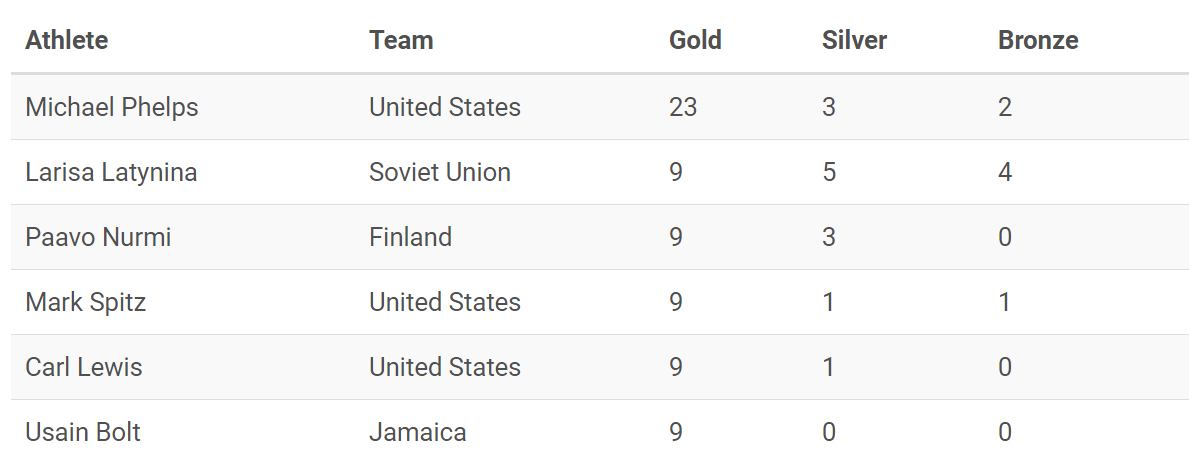
\includegraphics[scale=0.42,trim=0mm 0mm 0mm 0mm,clip]{images/table2.png} % left bottom right top
\end{center}
\caption{Athletes by the number of medals over the entire history of Olympic games}
\label{fig:case-table}
\end{figure}

% --------------------------------------------------------------------------------------------------

\section{Case study: Visualizing Olympic medalists}
\label{sec:impl}

We used The Gamma script with the pivot type provider to build an interactive web site 
(\url{rio2016.thegamma.net}) that visualizes a number of facts about Olympic medalists 
using the data set discussed in Appendix~\ref{app:olympics-csv} and used throughout this paper.
The web site lets the readers view and modify the source code and we also developed a number of
tools that make working with the source code easier, going beyond the basic auto-completion tooling
to enable dot-driven development as discussed in Section~\ref{sec:analysis-auto}. In this section,
we review our experience and outline some of the additional tools (available at 
\url{github.com/the-gamma}).

\subparagraph{Building tables and charts.} 
As part of the case study, we implement functions for building basic visualizations 
(table, column chart, pie chart and timeline) and we extended the host language with more advanced 
features that can be used to customize the displays. Building rich visualizations with the 
simplicity of the pivot type provider is an interesting future work. Figure~\ref{fig:case-table} 
shows a sample table, listing top athletes over the entire history of Olympic games.

The data transformation used to construct the table include the operations discussed in this paper
together with paging functionality and \qident{get the data} which returns the entire data set
of type \ident{Query}, as opposed to extracting a series with keys and values:
%
\begin{equation*}
\begin{array}{l}
\kvd{let}~\ident{data}~=~\ident{olympics}\\
\quad .\qident{group data}.\qident{by Athlete}\\
\qquad .\qident{sum Gold}.\qident{sum Silver}.\qident{sum Bronze}.\qident{concat Team}.\ident{then}\\
\quad .\qident{sort data}.\qident{by Gold descending}\\
\qquad .\qident{and by Silver descending}.\qident{and by Bronze descending}.\ident{then}\\
\quad .\ident{paging}.\ident{take}(10).\qident{get the data}\\[0.5em]
\ident{table.create}(\ident{data})
\end{array}
\end{equation*}

\noindent
The $\ident{table.create}$ operation on the last line generates a table based on the columns 
available in the data set. We omit the additional customization which specifies that medals should
be rendered as images. For most visualizations we built, the pivot type provider was expressive
enough to capture the core logic of the operation, but further joining of data was sometimes
needed. Possible extensions that would allow capturing those are discussed in 
Section~\ref{sec:further}.

% --------------------------------------------------------------------------------------------------

\begin{figure}[t]
\begin{center}
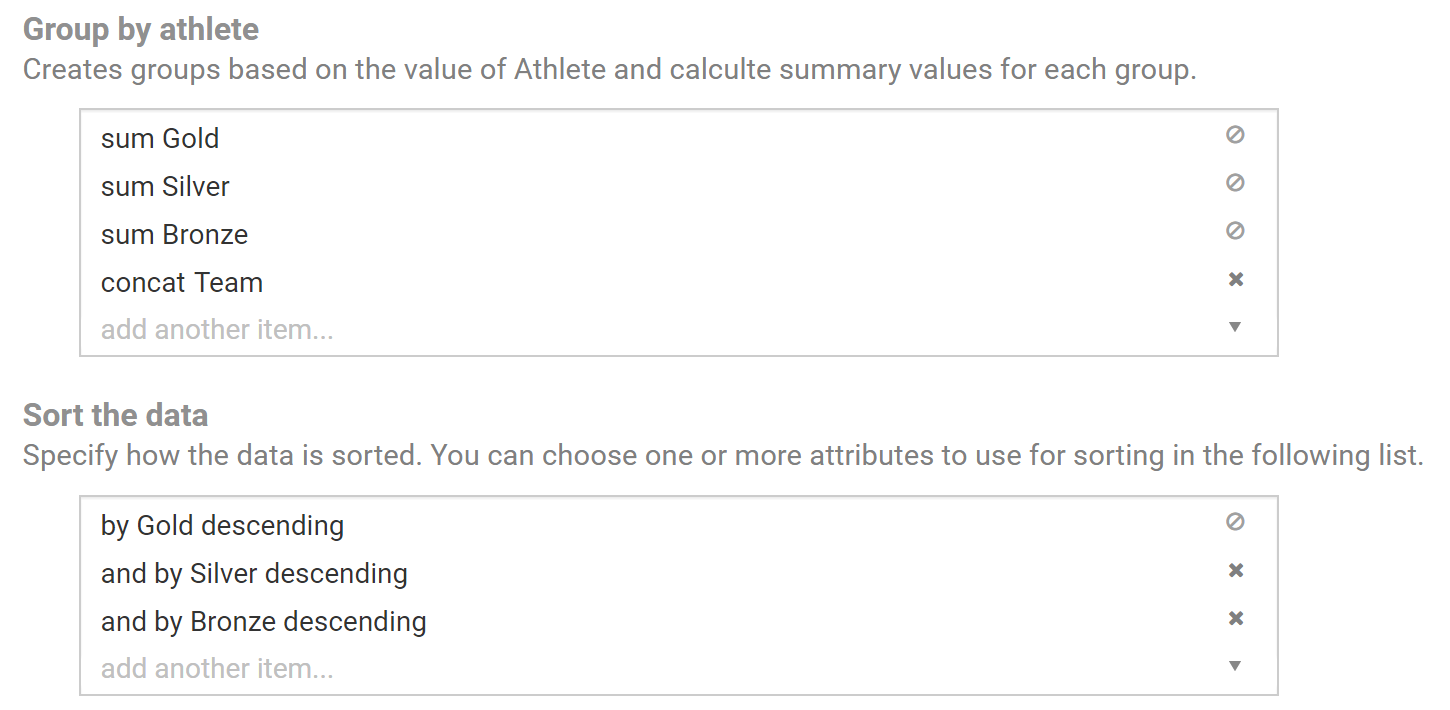
\includegraphics[scale=0.32,trim=0mm 0mm 0mm 0mm,clip]{images/options.png} % left bottom right top
\end{center}
\caption{User interface with automatically provided grouping and sorting options}
\label{fig:case-opts}
\end{figure}

% --------------------------------------------------------------------------------------------------

\subparagraph{Generating interactive user interfaces.}
Although the pivot type provider simplifies code needed for data exploration, not everyone will 
be able to write or modify source code. The simplicity of the host language makes it possible to  
automatically generate user interface that allows changing of some of the parameters of the program. 
Figure~\ref{fig:case-opts} shows an example for the above code snippet that we implemented as 
part of the visualization. 

The user interface lets the user choose aggregations to be calculated over a group and select 
columns used for sorting. It is generated automatically by looking for a specific pattern in the 
chain of member accesses -- we annotate members with annotations denoting whether a member is 
start of a list, list item or an end of a list. The editor then looks for parts of the chain of the
form $\qident{list start}.\qident{list item 1}.\qident{list item 2}.\qident{list end}$ and generates
a component that lets the user remove or add list items. An item cannot be removed if the operation
would break the code (e.g.~when it adds a member that is needed later) and items to be added
are chosen using available members (as in the standard auto-complete). The headers
shown in Figure~\ref{fig:case-opts} are provided as additional annotations attached to 
\qident{list start}.

% --------------------------------------------------------------------------------------------------

\subparagraph{Spreadsheet-inspired live editor.}
The third editor extension that we developed for the pivot type provider aims to bridge the gap 
between code and user interfaces. This is done through a direct manipulation editor \cite{directman} 
inspired by spreadsheet applications. When exploring data in a spreadsheet, the user can always see the 
data they work with and the results of an action will be immediately visible. This is not usually 
the case when writing code in text editor. However, when exploring data using the pivot type 
provider, the intermediate results can be calculated immediately using the sample data set provided 
when instantiating the refined version of the type provider with filtering support (Section~\ref{sec:pivot-filter}). 

The Figure~\ref{fig:case-ed} shows the sample expression (discussed above) in the live 
editor\footnote{The live editor can be tested live as part of the documentation for the 
JavaScript package at \url{thegamma.net}}.
Note that the selected part of code is the \qident{by Gold descending} identifier and so the 
preview shows results as computed at that point of the query evaluation. Athletes with largest number
of gold medals appear first, but silver or bronze medals are not yet used as secondary sorting keys
and so the secondary ordering is arbitrary.
As the user moves through the code, or writes the code, the live preview is updated accordingly.

Finally, the editor also makes it possible to modify the code through the user interface. The
``x'' buttons can be used to remove sort keys or transformations and ``+'' buttons (on the right)
can be used to add more transformations or to specify additional parameters within the ``then'' 
pattern. In case of sorting, this allows adding further sorting keys.

Unlike the user interface for modifying lists, the live editor works specifically with the pivot 
type provider. However, it still relies on the simple structure provided by the fact that entire 
transformation can be written as a single chain of member accesses. In particular,
we identify individual transformations (\qident{group by}, \qident{sort by}, etc.) and 
generate different user interface for specifying parameters of each transformation. For sorting, as 
shown in Figure~\ref{fig:case-ed}, the user can add or remove sort keys. For grouping 
or paging, the user interface lets the user choose the grouping key and the number of 
elements to take, respectively.

~

% --------------------------------------------------------------------------------------------------

\begin{figure}[t]
\begin{center}
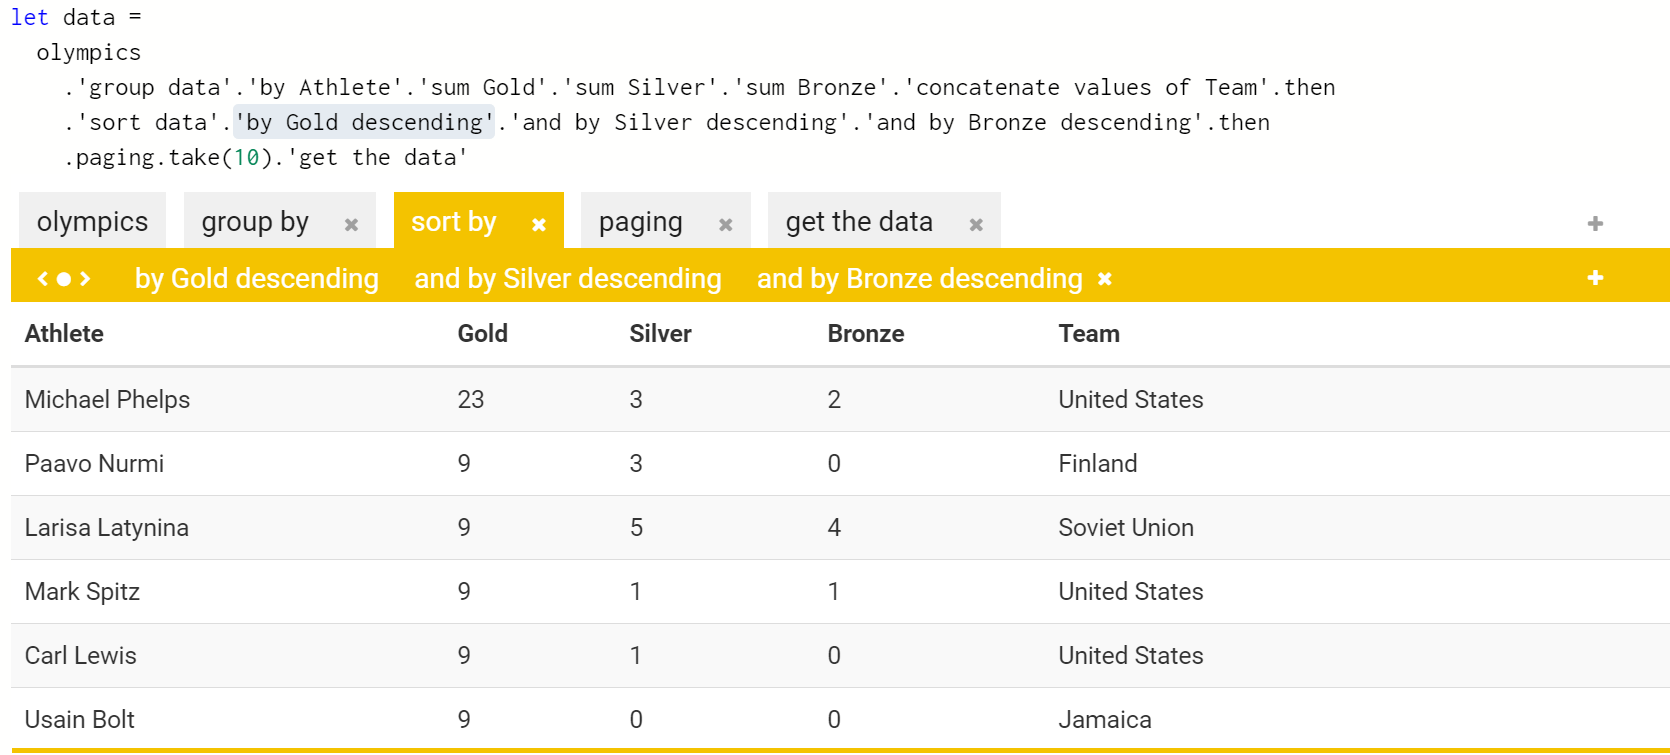
\includegraphics[scale=0.35,trim=0mm 0mm 0mm 0mm,clip]{images/pivot.png} % left bottom right top
\end{center}
\caption{Spreadsheet-inspired live editor for the pivot type provider}
\label{fig:case-ed}
\end{figure}


% ==================================================================================================

\section{Related and further work}

The technical focus of this paper is on the programming language theory behind the pivot type
provider (Section~\ref{sec:pivot}), but the paper also outlines interesting human-computer interaction 
aspects (Section~\ref{sec:impl}). We discuss further related directions in this
section before concluding.

\subsection{Further  work}
\label{sec:further}

The pivot type provider shows the feasibility of using dot-driven development as a mechanism behind 
simple programming tools for data exploration. Extending the mechanism to handle large and dirty 
datasets poses a number of interesting challenges.

\vspace{-0.25em}
\subparagraph{Scalability.} A benefit of our approach based on relational algebra, is that the 
query constructed by the pivot type provider can be translated to SQL and executed by a database 
engine. This means that evaluating the query over large data sets does not pose a problem. However,
the completion lists generated from data when filtering may require further consideration.

We plan to explore a number of possibilities such as grouping the values by a prefix (e.g.
\qident{starting with LO}.\ident{London} and \qident{starting with CA}.\ident{Cambridge})
or grouping the values by their frequency (for example, \qident{occurring less than 100 
times}.\ident{Grantchester} and \qident{occurring more than 10000 times}.\ident{London}). 
Such encoding makes it possible to scale to an arbitrary data size, provided that the backing 
data storage is equipped with an appropriate index.

\vspace{-0.25em}
\subparagraph{Expressivity.} 
The case studies presented in the paper show that the pivot type provider is practically useful in 
its current form, but we acknowledge that its expressivity is limited to simple queries.
Making the tool more expressive to allow tasks such as denormalisation, handling of missing values 
and dirty data is an important problem. 
Unlike data querying (which is captured by the relational algebra), there is no generally accepted 
``algebra of data cleaning'' and so more foundational work is needed, possibly building on 
from tools such as Wrangler \cite{wrangler} and PADS \cite{pads}. We believe that the 
``dot-driven development'' methodology can support richer languages and we intend to explore this
direction in the future.

\subsection{Related work}
\label{sec:related}

Our work builds on type providers, which have been pioneered in F\# \cite{inforich}.
The technical contributions are related to several works on type systems. This section
also gives an  overview of related work on human-computer interaction and commercial tools
for data visualization.

\subparagraph{Type providers.}
Type providers first appeared in F\# \cite{inforich} and can also be seen as a form of dependent 
typing \cite{idris-tp}; we take the opposite perspective and use type providers as a mechanism for 
implementing other type system features. Our focus on using type providers for describing 
computations is different from other type provider work \cite{fsdata,liteq,ageweb}, which focuses 
on mapping of external data into types. To our best knowledge, the Azure type provider \cite{azureprov} 
is the first type provider that provides members for specifying a restricted form of queries.

\subparagraph{Fancy types.}
The pivot type provider makes data exploration safer as it does not allow construction of invalid
queries. Alternative approach would be to use fancy types, such as those available in Haskell \cite{frames,fancytypes}. 
The approach sketched in Section~\ref{sec:columns-row} used row types and typestate or phantom types 
\cite{rowtypes,typestate,phanty}. The idea of using type providers to encode fancy types has also been
explored for session types \cite{sessionty,sessiontp} and it would be interesting to see whether
our approach can be applied in other areas such as web development \cite{urweb}.

\subparagraph{Human-computer interaction.}
We discussed how the pivot type provider simplifies the programming model (Section~\ref{sec:analysis}),
but it would be interesting to explore this aspect empirically through the perspective of HCI. 
The live editor shown in Section~\ref{sec:impl} offers a form of direct manipulation 
\cite{directman,directman2,dynamicq}. Unlike spreadsheets, we construct a transformation rather than
actually transforming data, which makes it more related to systems for query construction
\cite{spreadsheetalgebra,querydirect}. Our approach is somewhat different in that we see code 
as equally important to the direct manipulation interface.

\vspace{-0.25em}
\subparagraph{Relational algebra.}
Our operational semantics used to model data transformations (Section~\ref{sec:foo}) was based on 
relational algebra \cite{relalg,dbsys}, although our focus was on aggregation, which has been 
added to the core algebra in a number of different ways \cite{sumtables,datacube,relalg-alpha,relalg-sparql}.
The pivot type provider does not provide operations for joining data sets, which is an interesting
problem for further work as it requires extensions to the type provider mechanism -- the join
operation is parameterized by two data sets that are being combined.

\vspace{-0.25em}
\subparagraph{Commercial tools.}
There is a wide range of commercial tools for building dashboards and data visualizations such as
Microsoft Power BI \cite{powerbi}, Tableau \cite{tableau} and Qlik \cite{qlik}. Those allow users
to build data visualizations through a user interface and embedded scripting capabilities. 
The main difference from the pivot type provider is that none of these tools treats source code
as primary and so they do not provide the same level of reproducibility as scripts written using
the pivot type provider.


\section{Conclusions}
In this paper, we presented a simple programming language for data exploration. The language 
addresses two problems with the current tooling for data science. On one hand, spreadsheets are 
easy to use, but are error-prone and do not lead to reproducible scripts that could be modified
or checked for correctness. On the other hand, even simple data exploration libraries require 
the user to understand non-trivial programming concepts and offer only little help when writing 
data exploration code.

We reduce the number of concepts in the language by making member access (``dot'') the primary
programming mechanism and we implement type provider for data exploration, which offers 
available transformations and their parameters as members of a provided type. This leads to a 
simple language that can be well supported by standard tooling such as auto-completion. 
We also explore other possibilities for tooling enabled by this model ranging from 
simple interactive user interfaces to direct manipulation~tools.

The pivot type provider offers a safe and easy to use layer over an underlying relational algebra 
that we use to model data transformations. As a key technical contribution of this paper, we 
formalize the type provider and prove that queries constructed using the types it provides are 
correct. Achieving this property by other means would require a language with complex
type system features such as typestate and row types.

We believe that the simple programming model for data exploration presented in this paper can
contribute to democratization of data exploration -- you should not need to be an experienced 
programmer to build a transparent visualization using facts that matter to you!

\vspace{-0.25em}
\subparagraph{Acknowledgements.}
The author is grateful to Don Syme for numerous discussions about type providers, James
Geddes and Kenji Takeda for suggestions and useful references and to Mariana Marasoiu and
Alan Blackwell for ideas on human-computer interaction aspects of the work. Finally, thanks
to the anonymous reviewers for useful suggestions and corrections.

\bibliography{paper}

\appendix
\section{Sample of the Olympic medals data set}
\label{app:olympics-csv}

The data set used as an example in the case study discussed in Section~\ref{sec:impl} as well as
in the examples discussed throughout the paper is a single CSV file listing the entire history of
Olympic medals awarded since 1896. The data set can be found at \url{https://github.com/the-gamma/workyard}
together with scripts used to obtain it. The following is a representative example listing the
first 5 rows:
%
{\small
\begin{equation*}
\begin{array}{l}
\textbf{\sffamily {Games},{Year},{Discipline},{Athlete},{Team},{Gender},{Event},{Medal},{Gold},{Silver},{Bronze}}\\
\ident{Athens (1896)},\num{1896},\ident{Swimming},\ident{Alfred Hajos},\kvd{HUN},\ident{Men},\ident{100m freestyle},\ident{Gold},\num{1},\num{0},\num{0}\\
\ident{Athens (1896)},\num{1896},\ident{Swimming},\ident{Otto Herschmann},\kvd{AUT},\ident{Men},\ident{100m freestyle},\ident{Silver},\num{0},\num{1},\num{0}\\
\ident{Athens (1896)},\num{1896},\ident{Swimming},\ident{Dimitrios Drivas},\kvd{GRE},\ident{Men},\ident{100m freestyle for sailors},\ident{Bronze},\num{0},\num{0},\num{1}\\
\ident{Athens (1896)},\num{1896},\ident{Swimming},\ident{Ioannis Malokinis},\kvd{GRE},\ident{Men},\ident{100m freestyle for sailors},\ident{Gold},\num{1},\num{0},\num{0}\\
\ident{Athens (1896)},\num{1896},\ident{Swimming},\ident{Spiridon Chasapis},\kvd{GRE},\ident{Men},\ident{100m freestyle for sailors},\ident{Silver},\num{0},\num{1},\num{0}\\
\end{array}
\end{equation*} }

\noindent
The column names are the same as the column names used to generate the \ident{olympics} value using
the pivot type provider. The script to generate the file de-normalizes the \ident{Medal} column
and adds \ident{Gold}, \ident{Silver} and \ident{Bronze} columns which are numerical and can thus
be easily summed. When loading the data, we also transform country codes such as \kvd{GRE} to
full country names.

\end{document}
